%%%%%%%%%%%%%%%%%%%%%%%%%%%%%%%%%%%%%%%%%
% Beamer Presentation
% LaTeX Template
% Version 1.0 (10/11/12)
%
% This template has been downloaded from:
% http://www.LaTeXTemplates.com
%
% License:
% CC BY-NC-SA 3.0 (http://creativecommons.org/licenses/by-nc-sa/3.0/)
%
%%%%%%%%%%%%%%%%%%%%%%%%%%%%


%----------------------------------------------------------------------------------------
%	PACKAGES AND THEMES
%----------------------------------------------------------------------------------------

\documentclass[aspectratio=169]{beamer}



\DeclareMathOperator*{\argmin}{arg\,min}


%%%%%%%%%%%%%

\usepackage{hyperref}


\newcommand{\bi}{\begin{itemize}}
\newcommand{\ei}{\end{itemize}}
\newcommand{\m}{\item}
\newcommand{\be}{\begin{enumerate}}
\newcommand{\ee}{\end{enumerate}}
\newcommand{\al}{\alert}
\newcommand{\ul}{\underline}


\mode<presentation> {


\usetheme{Frankfurt}

% As well as themes, the Beamer class has a number of color themes
% for any slide theme. Uncomment each of these in turn to see how it
% changes the colors of your current slide theme.



}


%{%
%}

\setbeamercolor{section in head/foot}{bg=lightgray} %set the top navigation bar background color
\setbeamertemplate{footline}[frame number] % set frame page number only
\usepackage{appendixnumberbeamer} % total will not include appendix frame numbers 

\beamertemplatenavigationsymbolsempty



\usepackage{graphicx} % Allows including images
% graphicx also allows for resizebox
% graphicx also allows for \scalebox
\usepackage{caption}
\usepackage{subcaption} % packgage for subcaption in subfigures
% The subfig and subcaption packages can not be used in cooperation with each other. Instead, you can usecaption package with subfig to add some flavor to the captions and subcaptions
\usepackage{bm} % make bold math symbols
\usefonttheme{professionalfonts}
\usepackage{tabularx} % extra features for tabular environment
\usepackage{booktabs} % Allows the use of \toprule, \midrule and \bottomrule in tables
\usepackage{adjustbox} % allows adjustbox
\usepackage{amsmath}  
\usepackage{amsfonts}
\usepackage{hyperref} % package for hyper link

% the following hypersetup makes link blue
\hypersetup{
  colorlinks   = true, %Colours links instead of ugly boxes
  urlcolor     = blue, %Colour for external hyperlinks
  linkcolor    = blue, %Colour of internal links
  citecolor   = blue %Colour of citations
}


\usepackage{float} % make the table H effective
\restylefloat{table}
\usepackage{color, colortbl}
\usepackage{booktabs} % package for tex professional table
\usepackage{mathtools} % package for \coloneqq
\usepackage{multirow} % multirow for intuition page.

% make pdf dark mode

\usepackage{pifont}% http://ctan.org/pkg/pifont
\newcommand{\cmark}{\ding{51}}%
\newcommand{\xmark}{\ding{55}}%



\usepackage{tikz} % graph in latex
\usetikzlibrary{positioning,arrows.meta} %tikz diagram
\usepackage{pgfplots}
\pgfplotsset{compat=newest} %this setting allow node to go to the correct place
\usepgfplotslibrary{fillbetween}

% use the tikz external library to cache tikz drawings
\usetikzlibrary{external}
\tikzexternalize[prefix=tikz/,optimize command away=\includepdf]



\usepackage{natbib} % package for citation


% The subfig and subcaption packages can not be used in cooperation with each other. Instead, you can usecaption package with subfig to add some flavor to the captions and subcaptions


% define a comment line that does nothing to hide content
\newcommand{\comment}[1]{}
\newcommand{\lnb}[1]{%
  \ln\left(#1\right)%
}
\renewcommand{\baselinestretch}{1.0} %  scales the default interline space to 1.0 its default value. 

% define a comment that can scale the equation 
\newcommand\scalemath[2]{\scalebox{#1}{\mbox{\ensuremath{\displaystyle #2}}}}

%----------------------------------------------------------------------------------------
%	TITLE PAGE
%----------------------------------------------------------------------------------------

\title[Bitcoin, Blockchain, and Cryptocurrencies]{\huge{Bitcoin, Blockchain, and Cryptocurrencies} \\
\vspace{6mm}
\small{MGT 4074 Fintech \& Crypto Tokens, Fall 2025}
} % The short title appears at the bottom of every slide, the full title is only on the title page




\author[Joseph Hall]{Joseph Hall} % Your name
\institute[GT]{Georgia Institute of Technology} % Your institution as it will appear on the bottom of every slide, may be shorthand to save space
 % Your institution for the title page
 % Your email address
 
\date{September 10, 2025} 
 % Date, can be changed to a custom date if without date



%---------------------------------------------------------------------------
\begin{document}

\newcolumntype{d}[1]{D{.}{.}{#1}}


\begin{frame}
\titlepage % Print the title page as the first slide
\end{frame}


%----------------------------------------------------------------------------------------

%	PRESENTATION SLIDES
%----------------------------------------------------------------------------------------

%-----------------------------------------------



%---------------------------------------------------------------------
%---------------------------------------------------------------------
%---------------------------------------------------------------------
%---------------------------------------------------------------------



\begin{frame}{Welcome}

\begin{center}

    For Monday (9/15): \\
    Read the Bitcoin Whitepaper: \\ 
    \hyperlink{https://bitcoin.org/bitcoin.pdf}{https://bitcoin.org/bitcoin.pdf} \\ 
    \vfill
    Please create a MetaMask Wallet and fill out your \textbf{public} key in the Canvas quiz. \\ 
    \hyperlink{https://support.metamask.io/start/getting-started-with-metamask/}{https://support.metamask.io/start/getting-started-with-metamask/}
\end{center}
    \end{frame}



\begin{frame}
\frametitle{Roadmap}
\tableofcontents
\end{frame}

%------------------------------------------------



%------------------------------------------------
% insert table of content before each section or subsection
%------------------------------------------------
\AtBeginSection[]
{
\begin{frame}
\frametitle{Roadmap}
\tableofcontents[currentsection,currentsubsection]
\end{frame}
}
%------------------------------------------------

\section{In the News: Brazil Abandons Blockchain for CBDC}

\begin{frame}{Brazil Abandons Blockchain for CBDC}

Forbes: 

\begin{quote}
    Brazil’s Central Bank is abandoning the blockchain component of Drex, its ambitious central bank digital currency project.
\end{quote} \pause 

\begin{quote}
The project’s original vision was a two-tiered structure. The first monetary layer was to be an environment exclusively for transactions among authorized participants - specifically regulated financial institutions running nodes on the Central Bank-controlled network. The second would be tokenized bank deposits issued by regulated institutions to end customers. 
\end{quote}
    
\end{frame}

\begin{frame}{Discussion}

\textbf{Q}: What does CBDC stand for? \pause \textbf{A:} Central Bank Digital Currency \\ \pause 

\textbf{Q}: What does it mean for a CBDC to have a ``blockchain component?'' \\ \pause 
\textbf{A}: The full history of transactions using the CBDC would be cryptographically encoded in a series of ``blocks'', ``chained'' together with each block starting with a reference to the previous block. \\ \pause 

\textbf{Q}: What are the pros and cons of using a Blockchain, instead of a simple central database, to host CBDC?  \\ \pause 

\textbf{Benefits of Blockchain:} Decentralization, verifiability, trustlessness  \\ \pause 

\textbf{Drawbacks of Blockchain:} Computing power, privacy \\ \pause 

\textbf{TL;DR:} Brazil has decided not to record transactions of the ``Digital Real'' onto a blockchain. Instead, it will utilize a central database. 
    
\end{frame}

%---------------------------------------------------------------------
%---------------------------------------------------------------------
\section{Math}
%---------------------------------------------------------------------
%---------------------------------------------------------------------

\begin{frame}{Be Not Afraid}
    
\bi
\m Three math topics:
\bi
\m Hash functions
\m Digital signature schemes
\m Merkle Trees
\ei \pause
\m We do need to do \ul{some} math to understand what is really going on here
\bi
\m You are not expected to fully understand
\m I don't completely understand 
\ei \pause
\m Why am I teaching it then? \pause 
\bi
\m It's fun \pause 
\m The better you understand the math, the better you'll understand what is and is not technologically possible \pause 
\m You might be better than me at math \pause 
\m If a ``technical person'' knows this stuff worse than you, question their credentials 
\ei
\ei

\end{frame}



%------------------------------------------------
%------------------------------------------------
\subsection{Hash Functions}
%------------------------------------------------
%------------------------------------------------




\begin{frame}
\frametitle{A Philosophical Question\ldots}

Does true randomness exist in our physical universe? Or is everything predetermined?
\begin{center}
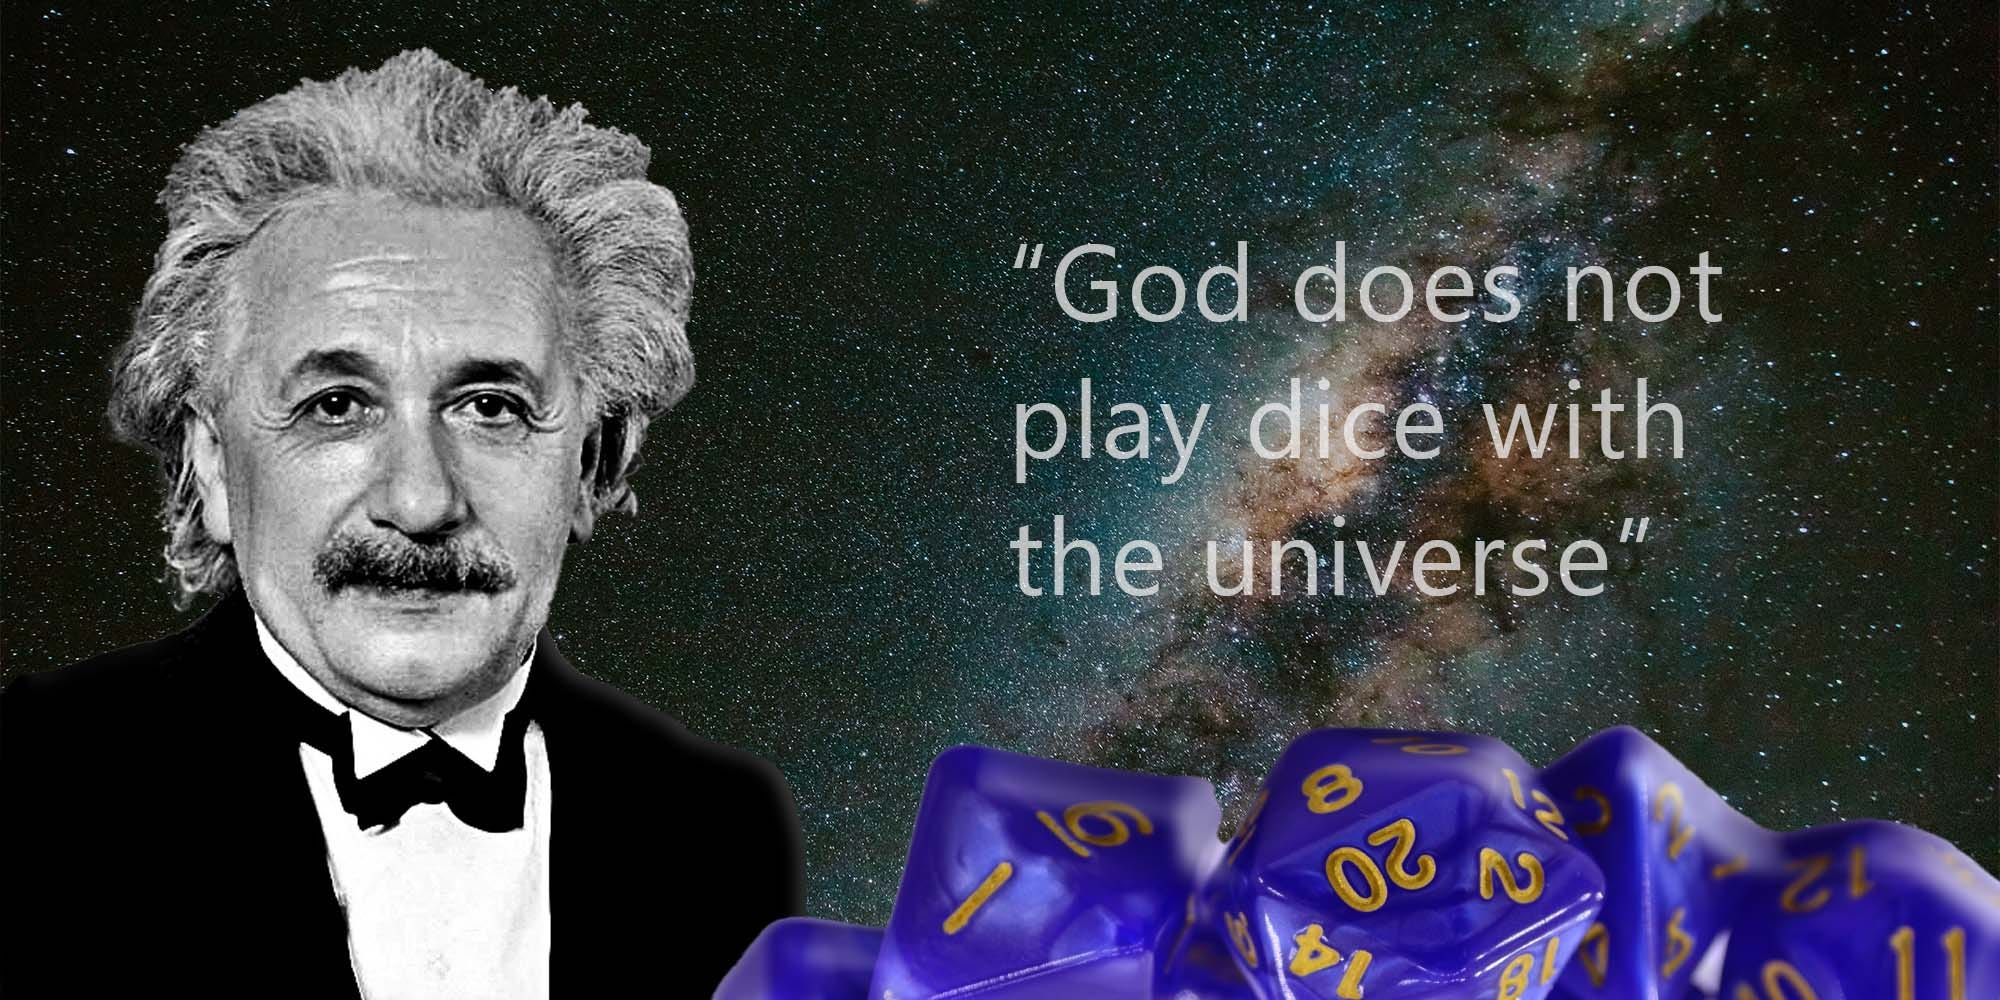
\includegraphics[width = 0.7\textwidth]{pics/einstein.jpg}
\end{center} \pause
\bi
\m If you think everything is predetermined, and we fully figure out the laws of physics, doesn't that mean we can predict the future? \pause
\m Anyone heard of the ``Three Body Problem''?
\ei

\end{frame}



\begin{frame}
\frametitle{Chaos}

\bi
\m Nature (and math) has many processes that are \textbf{chaotic}: \ul{deterministic}, but \ul{unpredictable}
\bi
\m Three-body problem
\m Physical dice, coins 
\m Which numbers are prime?
\ei  \pause
\m ``Deterministically'' driven by physics laws, but very sensitive to initial conditions, so from our perspective, \ul{as good as random} \pause 
\bi
\m We can simulate these (but always \emph{some} error) \pause 
\m But small changes in initial conditions change outcomes substantially
\m ``When a butterfly flaps its wings\ldots'' \pause 
\ei
\m Hash functions are \textbf{chaotic}: deterministic but unpredictable 
\bi 
\m \textbf{Deterministic}: The hash of a number never changes! 
\m \textbf{Unpredictable}: The hashes of two nearby numbers are \emph{very} far away, and there is \emph{no pattern} to how far 
\ei 
\ei

\end{frame}


\begin{frame}{A Chaotic Process}

\begin{center}
    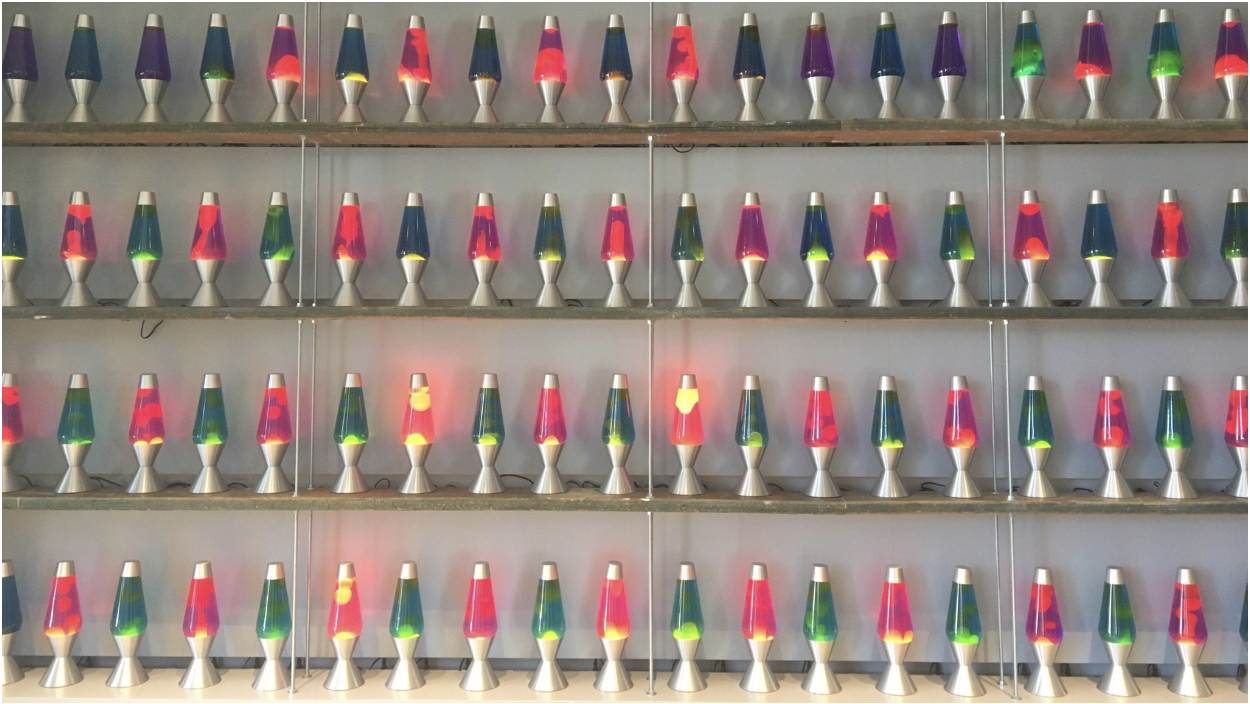
\includegraphics[width = .8\textwidth]{Screenshot 2025-01-28 at 6.23.12 PM.png}
\end{center}
    
\end{frame}


\begin{frame}{A Chaotic Process}

\begin{center}
    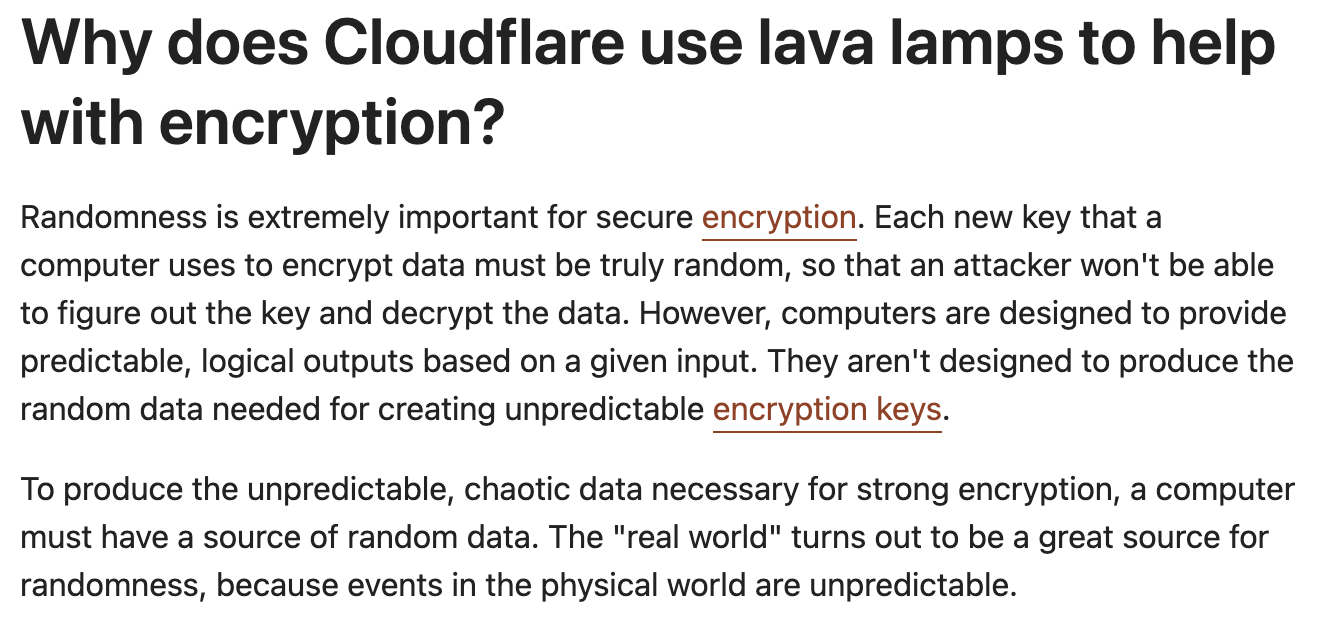
\includegraphics[width = .9\textwidth]{Screenshot 2025-01-28 at 6.23.04 PM.png}
\end{center}
    
\end{frame}


\begin{frame}
\frametitle{Chaotic Functions}

\bi
\m A \textbf{hash function} takes some input string, and ``chaotically'' spits out an output string. \href{https://emn178.github.io/online-tools/sha256.html}{Demo}
\m Servers (to which you log in) store hashes, not passwords! \pause 
\m Intuitively, ``chaos'' gives us some very nice properties
\bi
\m \textbf{One-way:} Can calculate outcomes, but can't back out initial conditions
\m \textbf{Collision Resistance:} Lots of outcomes are possible, so two initial conditions rarely result in same outcome (a ``collision'') 
\ei \pause
\m Practically: do some silly \ul{deterministic} operation, a lot of times, until all the input information is scrambled:
\bi
\m Convert text to binary numbers, 1101010\ldots
\m Flip the 4th, 13th, 18th from 1 to 0, or 0 to 1\ldots
\m Make 5th, 17th, and 12th number vote on whether 3rd is 0 or 1\ldots
\m Move 1st to 2nd, 2nd to 3rd\ldots 64th to 1st\ldots
\ei \pause
\m Tl;dr, record your kid doing random stuff, and repeat it a lot of times
\ei

\end{frame}

\begin{frame}\frametitle{Hash Functions}

A cryptographic hash function is a mapping H : M → D from a set M of possible messages of any length to a set D of digests, for example the set of strings of 0s and 1s of a fixed length, such as 256. See \href{https://www.youtube.com/watch?v=0WiTaBI82Mc}{Ramzan (2012)}. 
\vfill \pause 
For usefulness, a cryptographic hash function H should be easily computable and, among other properties, be: 
\begin{enumerate}
    \item \textbf{Collision resistant}, meaning that H is “nearly injective.” That is, it should be extremely \ul{rare} to have H(x) = H(y) unless x = y.\pause 
    \item \textbf{Difficult to invert}. That is, it should be extremely hard to guess x, or properties of x\footnote{digital signature schemes do preserve \ul{some} properties of x as we will see}, from H(x).\pause 
    \item \textbf{Extremely sensitive}. Even small changes in the message should usually produce large changes in the digest.  \pause 
\end{enumerate}
In \textbf{digital signature schemes} (as we will see), a ``digest'' is a \textbf{signed message}. 
\end{frame}


\begin{frame}{Collision Resistance and Invertability}

\textbf{Question}: Suppose a function H maps the integers {1, 2, 3, 4, 5, 6} to the integers {0, 1, 2, 3, 4, 5} by letting H(x) = x - 1. For example, H(5) = 4. Is H collision resistant? \pause 
\vfill 
\textbf{Answer}: Yes, it is. Observe that $H(x) - H(y) = x - y$ in this case, so if $x \ne y$, then $H(x) \ne H(y)$ \pause 
\vfill 
\textbf{Question}: is $H(.)$ difficult to invert? \pause 
\vfill 
\textbf{Answer}: No, it is easy to invert. In this case $H^{-1}(x) = x + 1$ \pause \vfill 
\textbf{Question}: is $H(.)$ a useful cryptographic \textbf{hash function}? \pause 
\vfill 
\textbf{Answer}: No, hash functions must be hard to invert. 
    
\end{frame}


\begin{frame}
\frametitle{Hash Functions}

In blockchains, hash functions have two main uses:

\bi
\m By publishing $y=H(x)$, anyone can check that they know the real $x$ \ul{without $x$ ever becoming public information} \pause 
\bi
\m Easy to compute $H(x)$ given $H(\cdot)$ and $x$ \pause 
\m If someone changes $x$ to $\tilde{x}$, even by one letter, $H(\tilde{x})$ will be very different!
\m Used in checksums for file downloading \pause 
\ei
\m Application: \textbf{Mining and proof-of-work}
\bi 
\m No way to discover $x$ given $H(x)$ beside \textbf{brute force}! \pause 
\m The Secure Hash Algorithm 1 (``\textbf{SHA1}'') takes between $2^{63}$ - $2^{80}$ evaluations to find a collision ($x,y$ such that $H(x)=H(y)$) (depending on how clever you are) \pause 
\m Bitcoins are mined by brute-forcing hashes to find $x$s that produce $H(x)$ with leading zeroes. 
\ei 
\ei

\end{frame}


\begin{frame}
\frametitle{Modular Arithmetic}


\begin{footnotesize}

\centering
\begin{tabular}{|c|c|c|c|c|c|c|c|c|c|}
	\hline 
	Powers of 3 & $3^{1}$ & $3^{2}$ & $3^{3}$ & $3^{4}$ & $3^{5}$ & $3^{6}$ & $3^{7}$ & $3^{8}$ & $3^{9}$\tabularnewline
	\hline 
	Value & 3 & 9 & 27 & 81 & 243 & 729 & 2187 & 6561 & 19683\tabularnewline
	\hline 
	Closest multiple of 7 & 0 & 7 & 21 & 77 & 238 & 728 & 2184 & 6559 & 19677\tabularnewline
	\hline 
	Remainder div. 7 & 3 & 2 & 6 & 4 & 5 & 1 & 3 & 2 & 6\tabularnewline
	\hline 
\end{tabular}
\end{footnotesize}
\bi
\m We use $x\mod y$ to mean, ``remainder of $x$ when divided by $y$'', like:
\[
81\mod7=4
\]
\m In python, $x\mod y$ is just $x\ \%\ y$
\m In R, it's $x\ \%\%\ y$

\ei

\end{frame}


\subsection{Digital Signatures}

\begin{frame}
\frametitle{How do I prove that I signed something?}

Requirements:
\bi
\m JPH has a public key everyone knows
\m JPH has a private key only JPH knows
\bi 
\m \textbf{Non-invertability} means the public key doesn't reveal the private key \pause 
\ei 
\m JPH can ``sign'' messages: use the private key to alter the message in a way that \ul{proves} JPH created his public key 
\m Public key allows \textbf{verification}, but not \textbf{signature production} \pause 
\bi
\m Using public key, anyone can verify signature correctness: JPH used his private key to sign the message \pause 
\m But, using the public key, can't generate new valid signatures
\ei
\ei

\end{frame}


\begin{frame}{Digital Signatures, Formally}

A \textbf{Digital Signature Scheme} is a combination of \ul{Three Functions}: 

\bi 
\m A function to generate \textbf{Public Keys}: $PrK \Rightarrow PuK$ \pause 
\m A function to generate \textbf{Signed Messages}: $(PrK, M) \Rightarrow M'$ \pause 
\m A function to \textbf{Verify} signed messages: $(PuK, M, M') \Rightarrow \{0,1\}$ \pause 
\ei 

These functions ($\Rightarrow$) are \ul{one-way}, \ul{chaotic} functions! \pause \\
In Bitcoin, these ``messages'' encode a list of transfers of blocks from one owner to another! 

\end{frame}

\begin{frame}{Digital Signature Schemes, Visually}

\begin{center}
    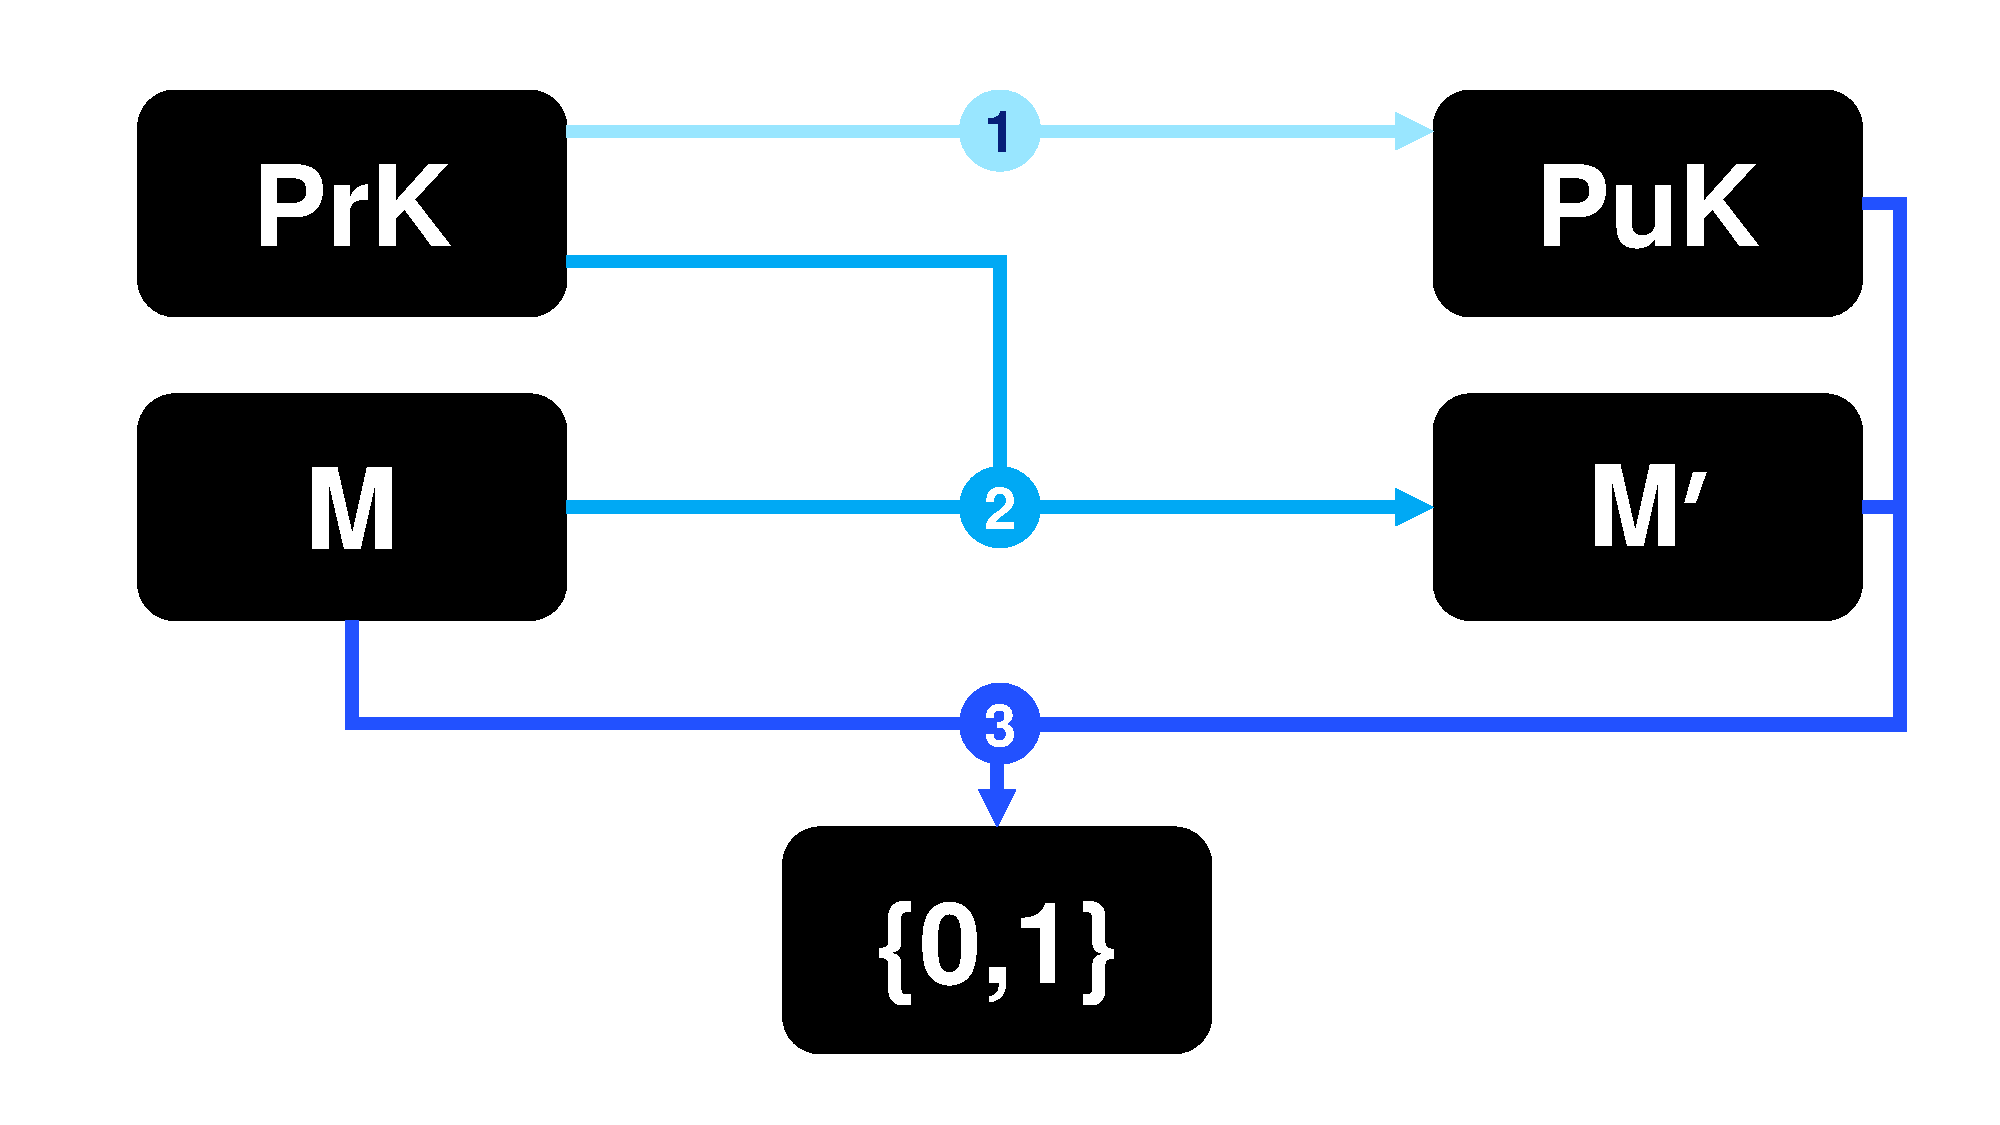
\includegraphics[scale = 0.3]{pics/Financial Technology Timeline for Joseph slide 2.pdf}
\end{center}
    
\end{frame}

\begin{frame}{Ok, but how do these signatures actually \ul{work}?}

\href{https://ece.gatech.edu/courses/ece6280}{ECE 6208} teaches this; it is beyond my own understanding. 

\vfill 
The easiest to implement from scratch, that I'm aware of, is called \href{https://www.geeksforgeeks.org/elgamal-encryption-algorithm/}{ElGamal.} \pause (``The Beauty'' in Arabic) 
    
\end{frame}


\begin{frame}{Welcome! Today is Monday 9/15}
    There is a reading quiz today on the Bitcoin Whitepaper. \\ \vfill 
    Midterm 1 will be discussed at the start of class. Your copies will be distributed at the end of class. \emph{If you think you may appeal your score}, you must inform me at that time so I can photograph your exam and ensure you do not alter it.\\ \vfill 
    Homework 1 has been posted to Canvas. As of today you will know everything you need to know to complete it. It is due at the start of class 7 days from today. 
\end{frame}


\begin{frame}{Midterm 1 Post-Mortem}

Short Answer Question 1: The No-Trade Theorem. \\ 

\textbf{Assumptions:} 
\begin{itemize}
    \item Heterogeneous information (in no particular direction!) 
    \item Common preferences (everyone values the same cash flows the same) 
    \item (There is also an assumption of rational expectations, but that was not in the slides nor necessary to state for full credit on the exam) 
\end{itemize} \pause 

The \textbf{result of those assumptions} is that no trade should take place! \\ 
The intuition is that being offered a trade is sufficient reason to reject it, if there are no positive-sum trades! \\ 
The take-away is that trade in financial markets \textbf{must} be based on differences in preferences: e.g. someone who needs money today trades with someone who needs money tomorrow. 
    
\end{frame}

\begin{frame}{Midterm 1 Post-Mortem}

Short Answer Question 2: \emph{Seignorage} is the profit from printing money. \\ \vfill 

\begin{itemize}
    \item \textbf{Specie} is a naturally-scarce material. 
    \begin{itemize}
        \item Seignorage can be earned through \textbf{coinage} and increased through \textbf{debasement}
    \end{itemize}
    \item \textbf{Fiat} is a currency on which the government enforces coordination. 
    \begin{itemize}
        \item Seignorage is \emph{maximized} with this form of currency 
    \end{itemize}
    \item \textbf{Crypto} is a currency secured with cryptography
    \begin{itemize}
        \item The most valuable cryptocurrency, \textbf{Bitcoin}, has no seignorage 
        \item A cryptocurrency can be designed to give seignorage to its creator (this was not necessary to state in order to earn full credit). 
    \end{itemize}
\end{itemize}

\end{frame}


\begin{frame}{In the News: Stablecoin Price War}

From Bloomberg's Matt Levine: 

\begin{center}
    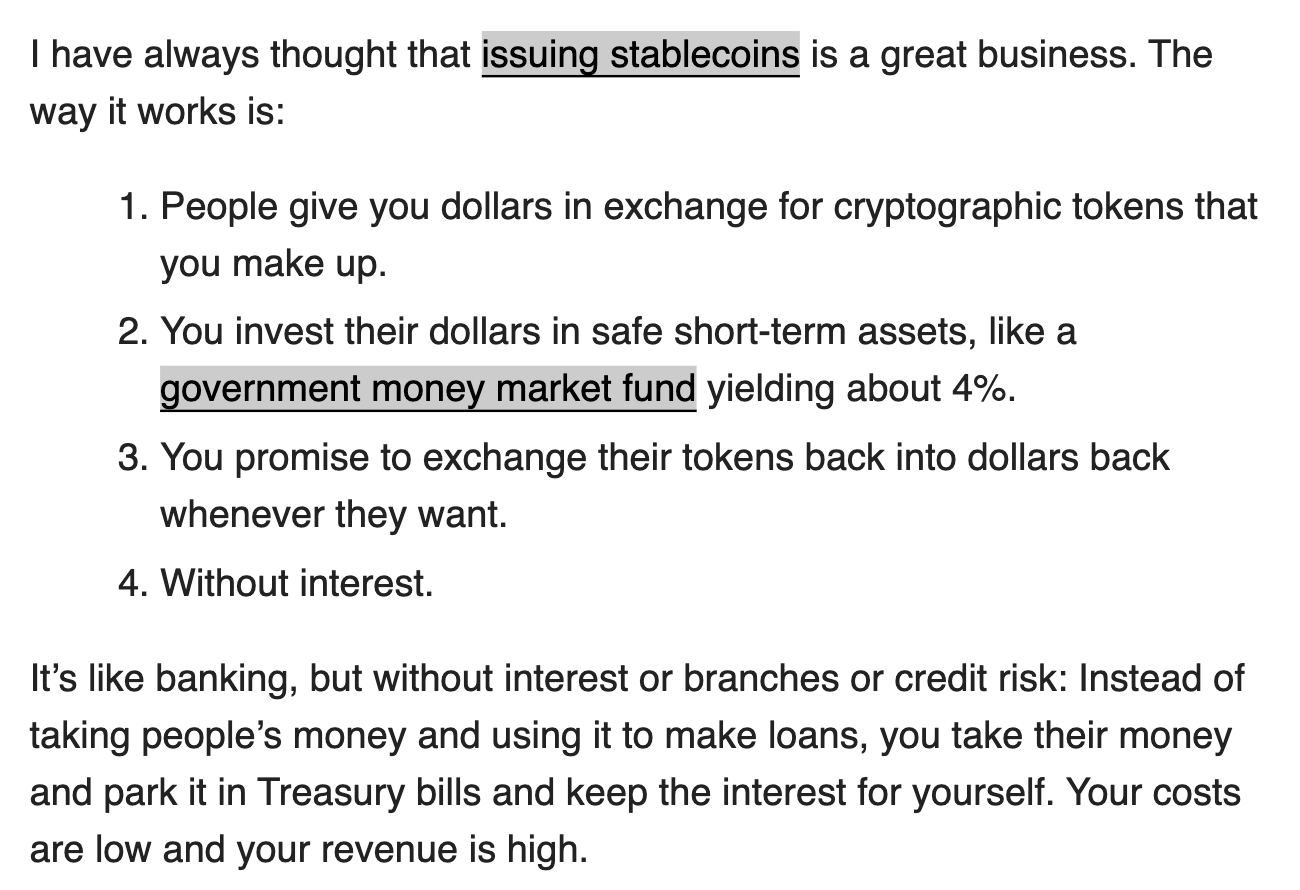
\includegraphics[height = .7\textheight]{levine_1.png}
\end{center} \pause 
\end{frame}

\begin{frame}{In the News: Stablecoin Price War}

\textbf{Q:} What incentives does this create for stablecoin issuers? \pause \\ 
\textbf{A:} Incentives to pay interest and attract more deposits \pause \\ 
\textbf{Q:} What is the problem with this plan? \pause \\ 
\textbf{A:} The GENIUS Act prohibits interest on stablecoins! \pause \\ 
\textbf{Q:} So what do they do? \pause \\ 
\textbf{A:} They pay a fee to exchanges to make their stablecoin the native stablecoin of the exchanges. The exchanges then rebate that fee to the end users, running around the GENIUS Act regulation. \pause \\ 
\textbf{Q:} Why don't the regulators like this outcome? \pause \\ 
\textbf{A:} If deposits flow out of banks and into stablecoins, we will lose the liquidity-transforming, loan-supplying function of banks! 
    
\end{frame}


\begin{frame}{In the News: Stablecoin Price War}

So where does this leave us? 

\begin{center}
    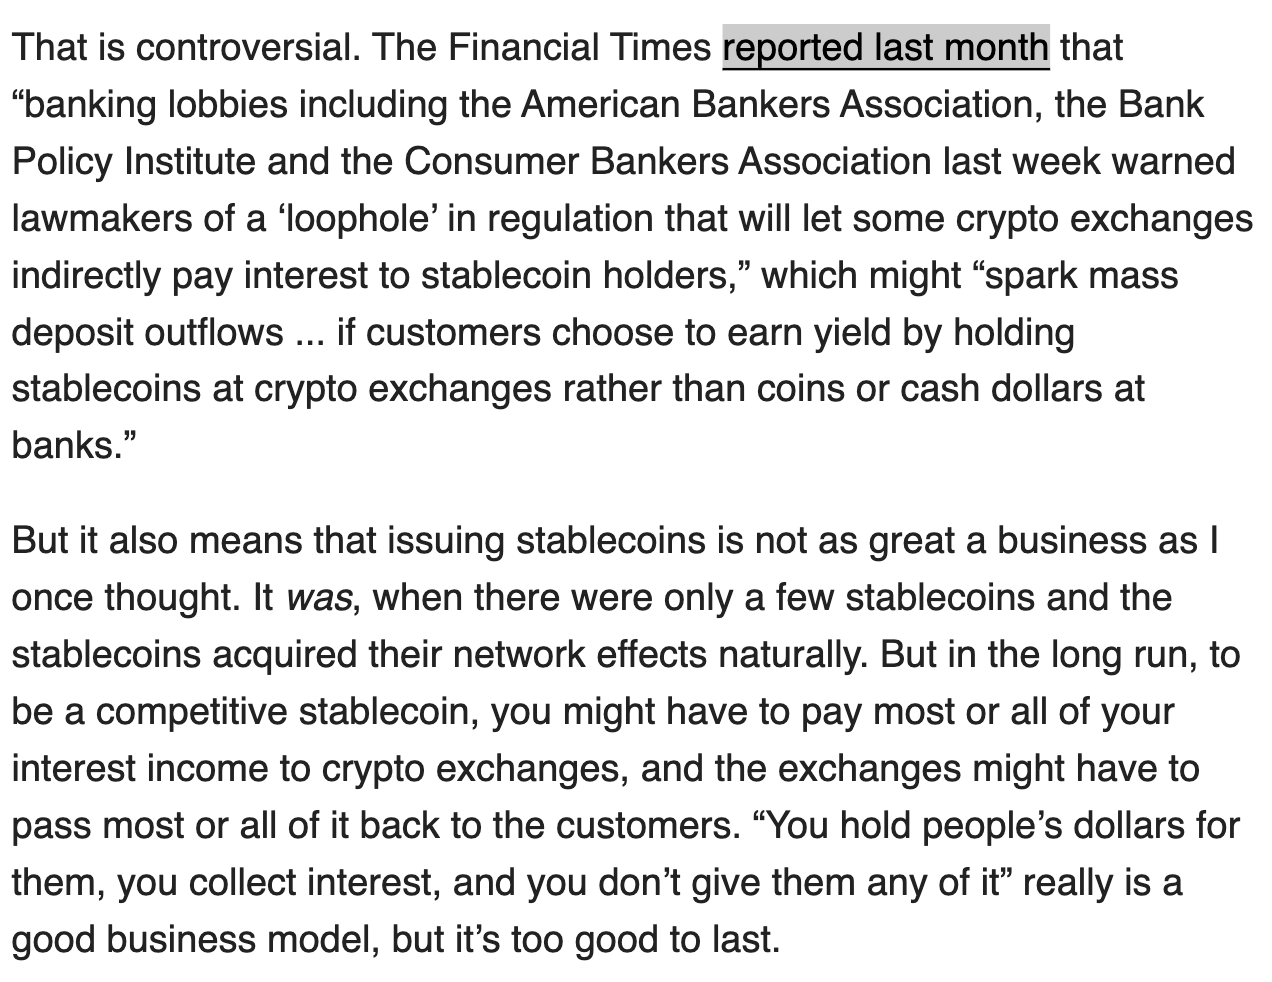
\includegraphics[height = .8\textheight]{levine_2.png}
\end{center} \pause 
    
\end{frame}


\subsection{Merkle Trees}

\begin{frame}{Uses of Merkle Trees}

A \hyperlink{https://decentralizedthoughts.github.io/2020-12-22-what-is-a-merkle-tree/}{Merkle Tree} is a way of \ul{efficiently} storing the required information to ensure that a set of documents or messages have not been tampered with or corrupted. \pause 
\vfill 
Merkle Trees are used in many applications to solve problems such as:

\bi 
\m Maintaining integrity of files stored on Dropbox.com, or \emph{file outsourcing}
\m Proving a transaction between Alice and Bob occurred, or \emph{set membership}
\m Transmitting files over unreliable channels, or \emph{anti-entropy}
\ei 
    
\end{frame}

\begin{frame}{Construciton of Merkle Trees}

Start with, say, 8 files $(f_1...f_8)$, and a hash function $H(.)$ \vfill \pause 

Start by hashing each file $H(f_i)$: 

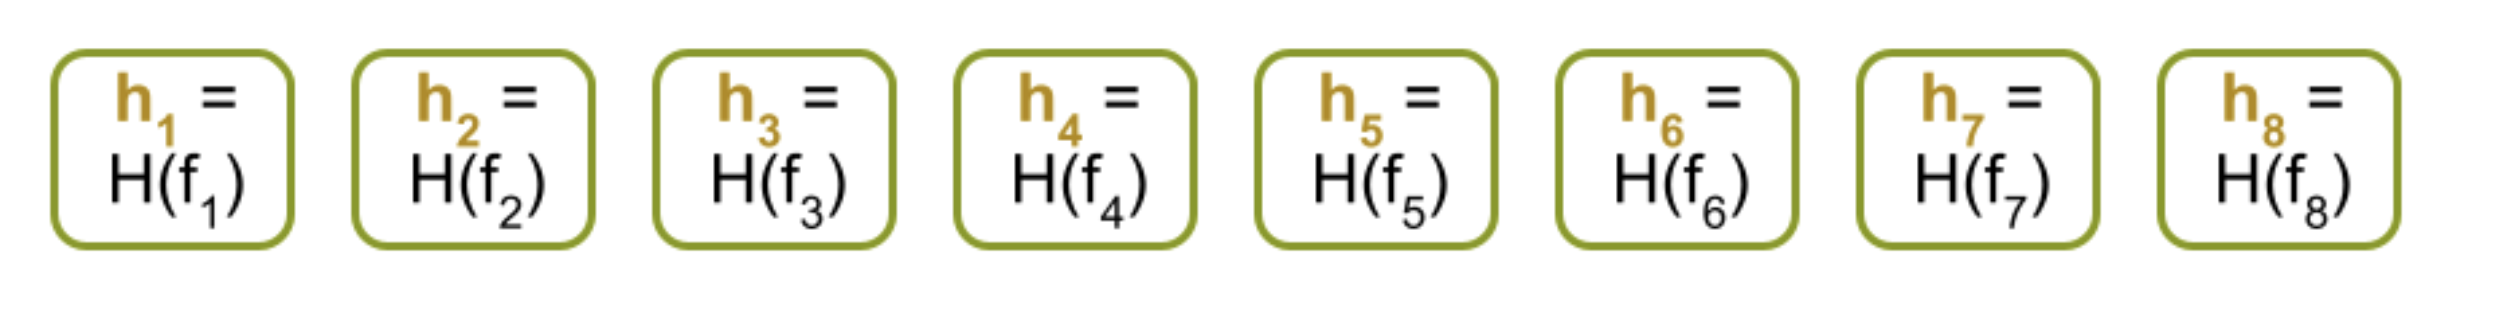
\includegraphics[scale = 0.3]{Screenshot 2025-01-27 at 7.38.00 PM.png}
    
\end{frame}

\begin{frame}{Construction of Merkle Trees}

Then, create the second layer of the tree by hashing adjacent nodes \ul{together} (this can be as simple as concatenating them!) 

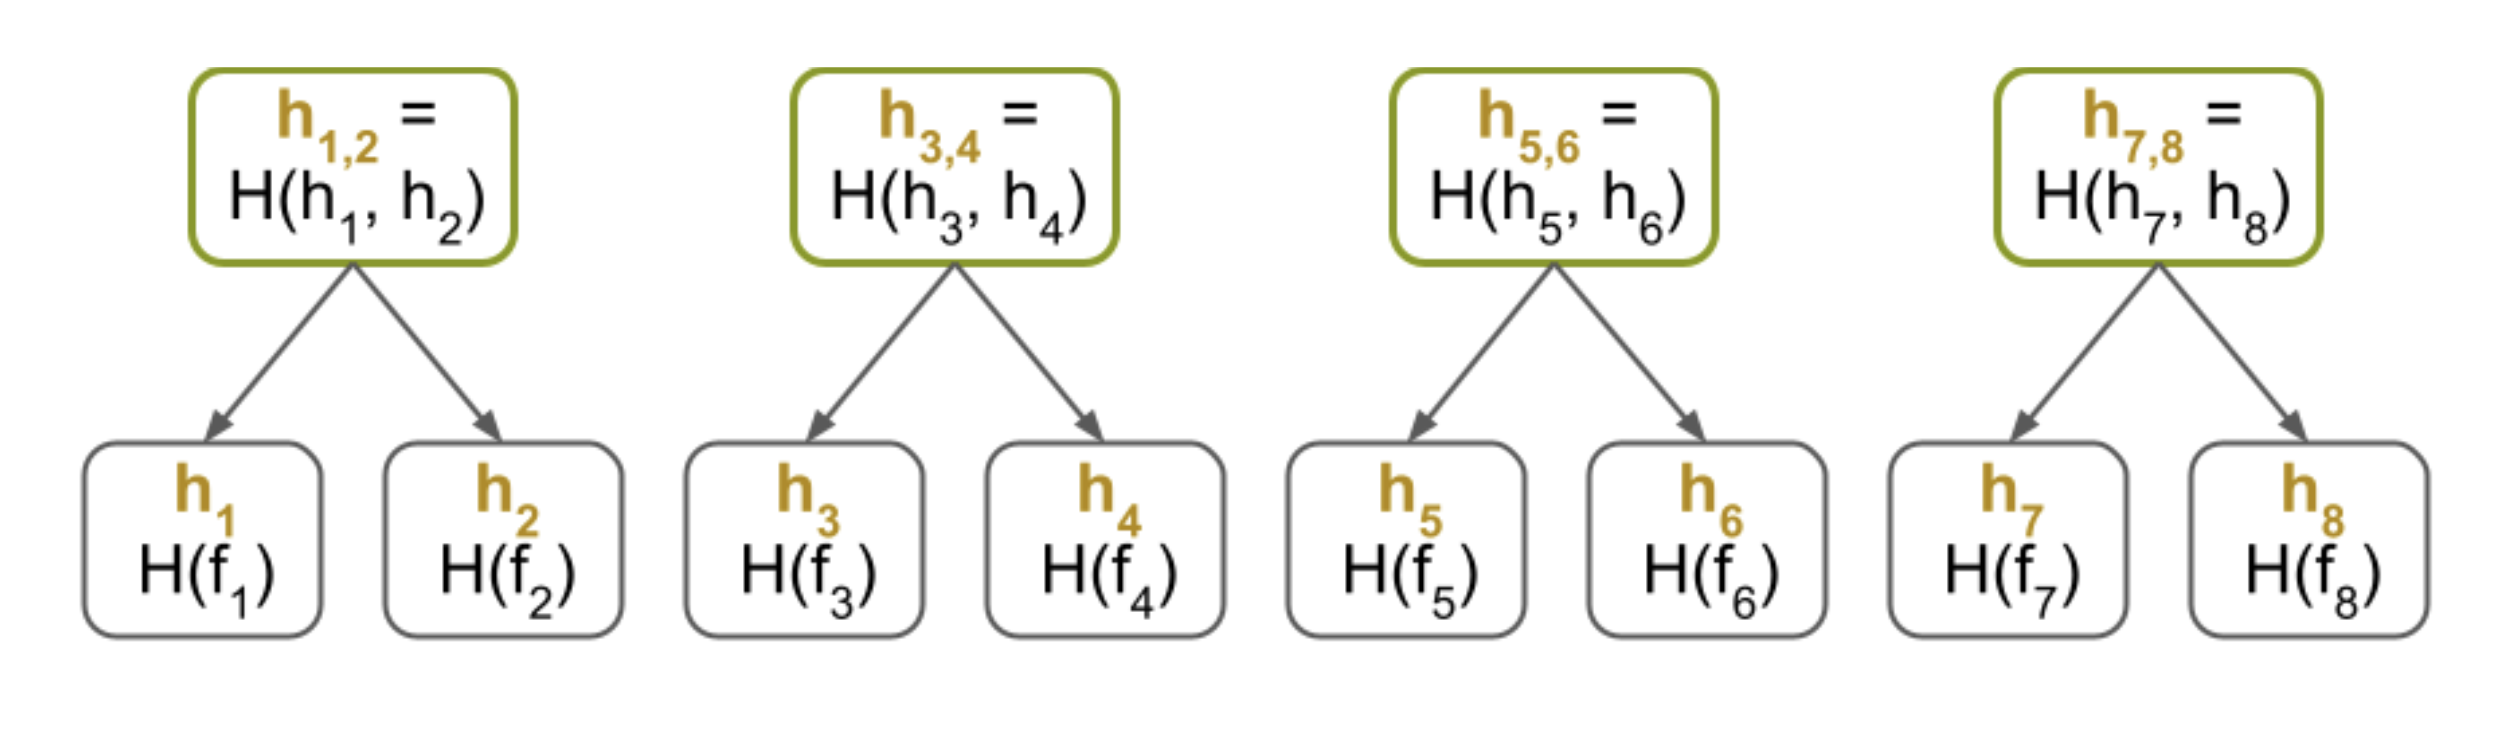
\includegraphics[scale = 0.3]{Screenshot 2025-01-27 at 7.40.09 PM.png}
    
\end{frame}

\begin{frame}{Construction of Merkle Trees}

Continue until you have created an entire ``tree'': 
\begin{center}
    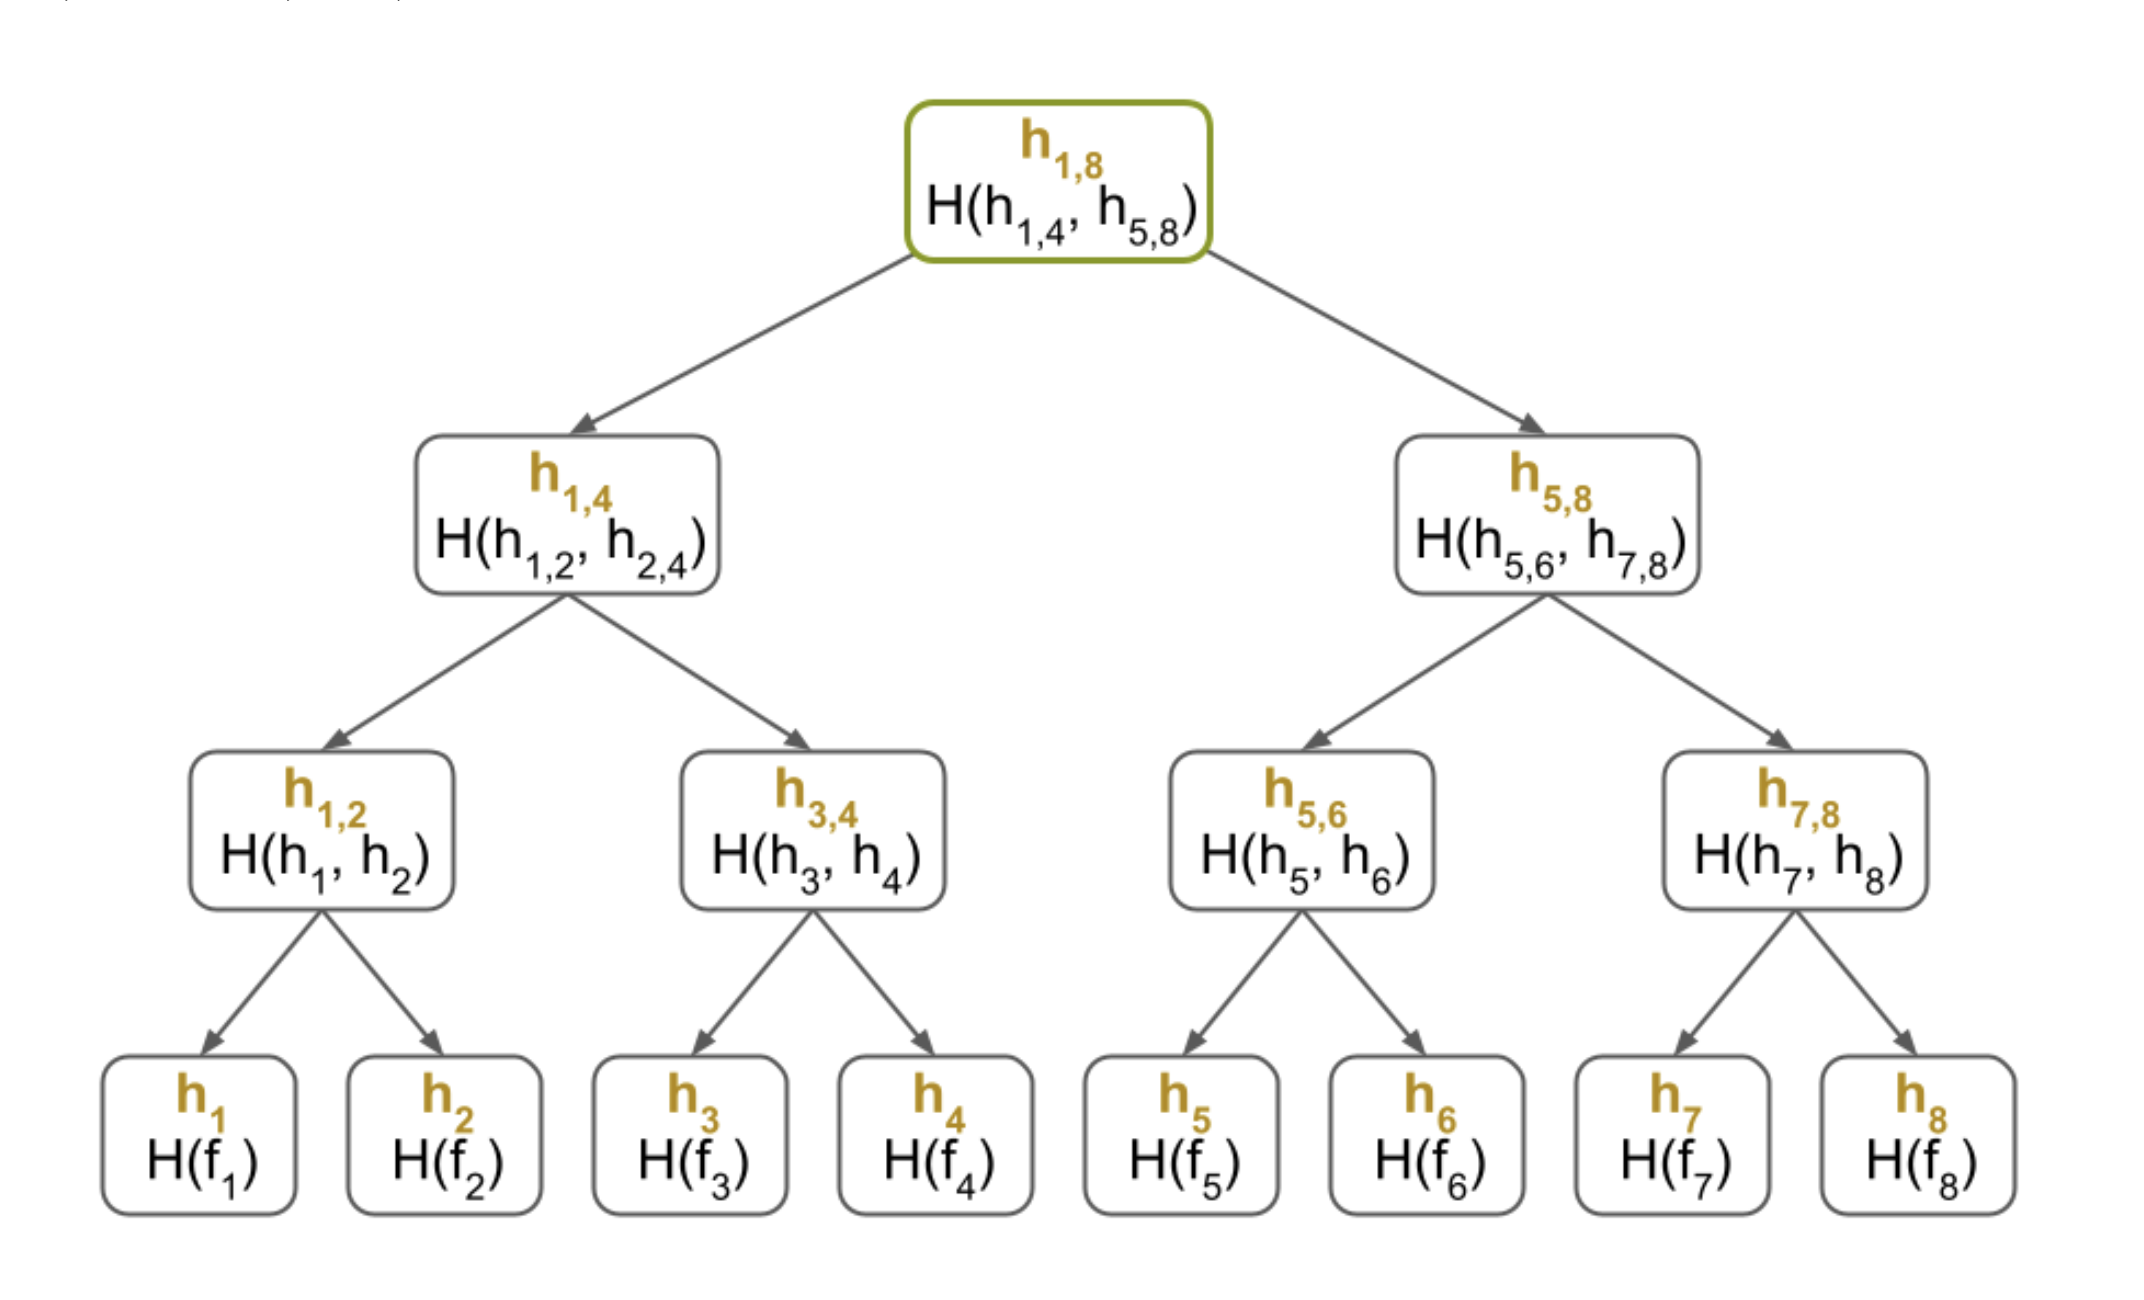
\includegraphics[scale = 0.3]{Screenshot 2025-01-27 at 7.43.10 PM.png}
\end{center}

\end{frame}

\begin{frame}{Construction of Merkle Trees}

\textbf{Question}: Why is this tree upside-down? \pause 

\textbf{Answer}: Because Computer Scientists have never gone outside, a necessary prerequisite to see a real tree 
    
\end{frame}

\begin{frame}{Verification with Merkle Trees}

Upload your files $(f_1...f_8)$ \textbf{and} your Merkle Tree to Dropbox, storing \ul{only} the \textbf{Merkle Root} $h_{1,8}$ locally. \pause \vfill 
Later, ask for the file you want, say $f_3$, but make sure to also ask for the \textbf{Merkle Proof}: the hashes needed to compute $h_{1,8}$ from the desired \textbf{Merkle Leaf} ($f_3$)

\end{frame}

\begin{frame}{Verification with Merkle Trees}

The \textbf{Merkle Proof} lets you verify that you downloaded the real, original $f_3$: 

\begin{center}
        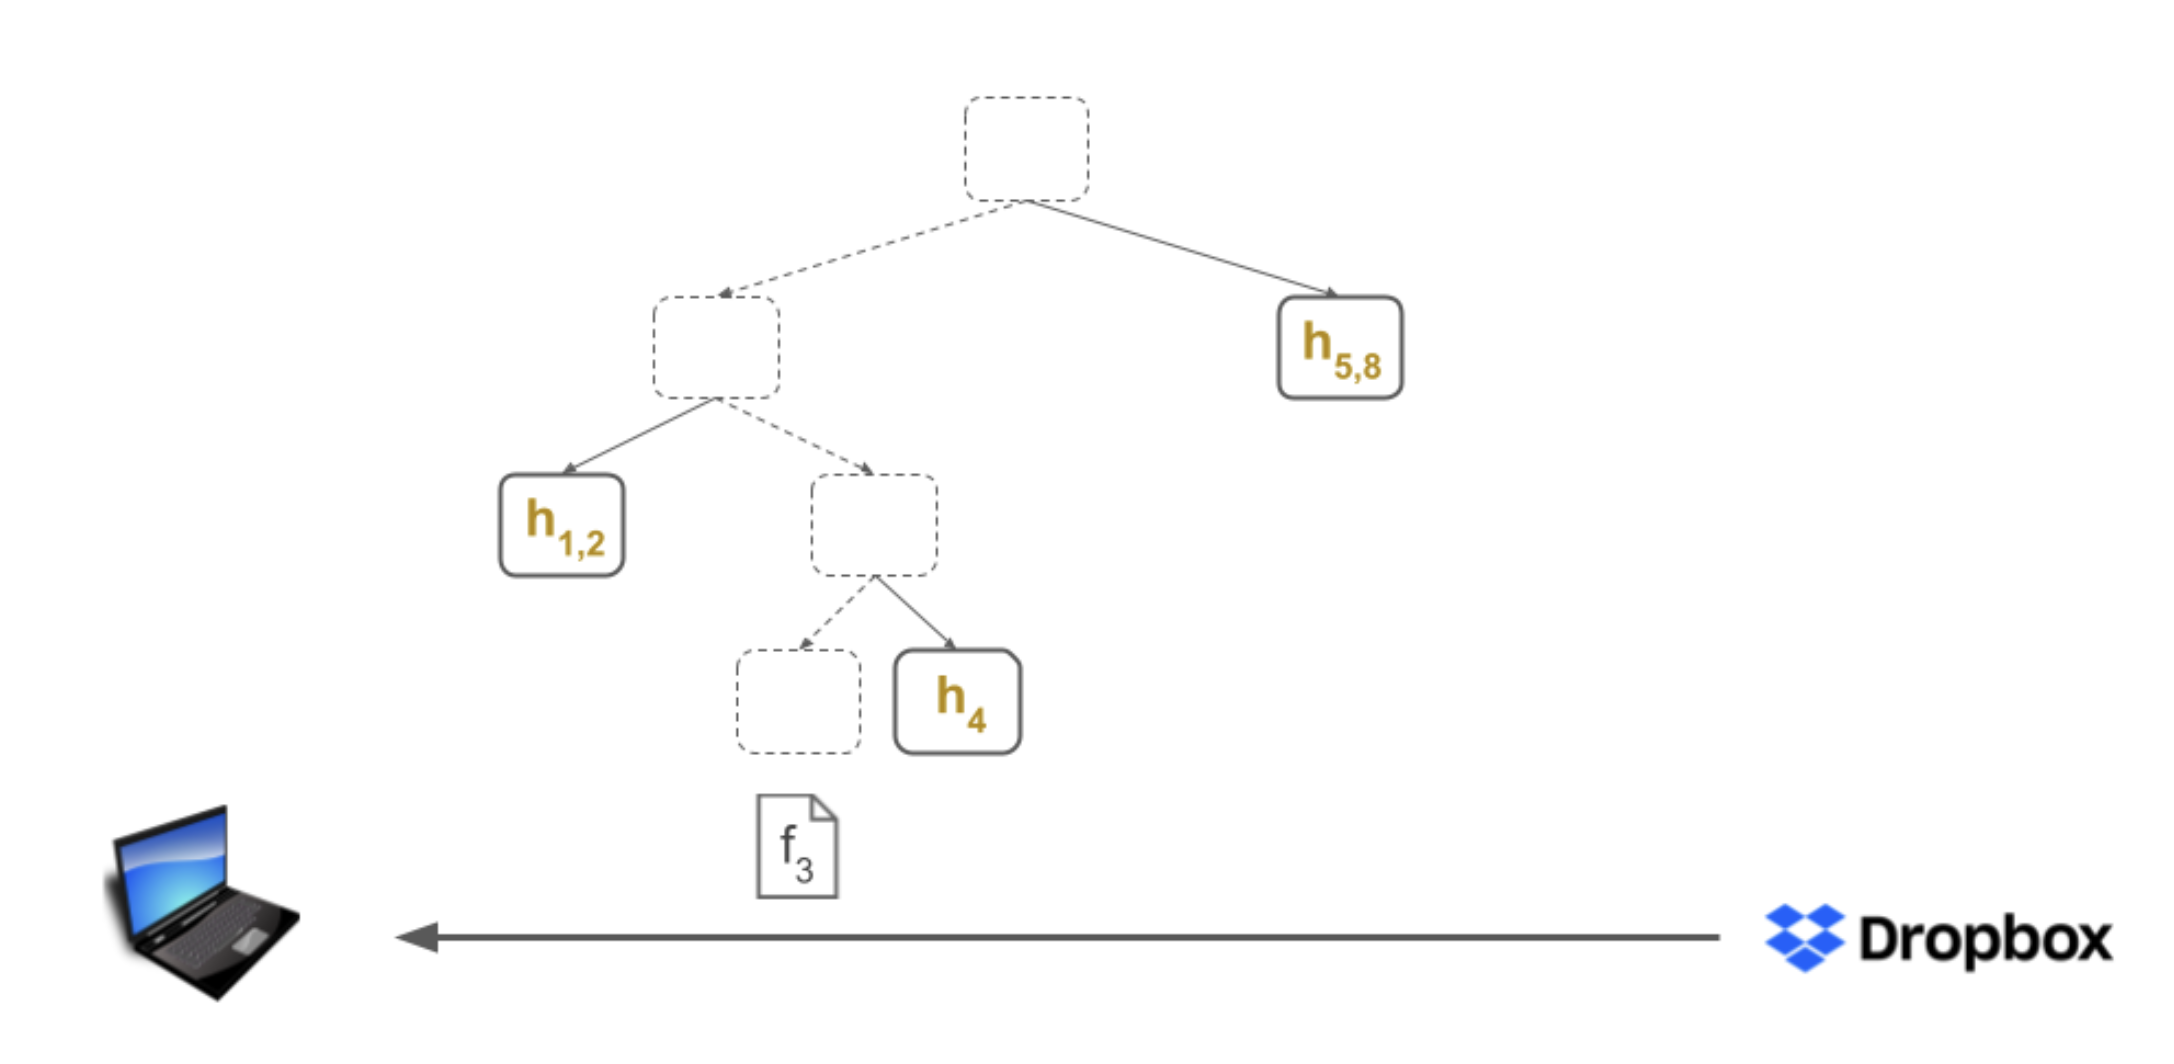
\includegraphics[scale = 0.3]{Screenshot 2025-01-28 at 1.46.09 PM.png}
\end{center}
    
\end{frame}

\begin{frame}{Advantages of Merkle Trees}

\textbf{Question}: Why not just store the hash of every file? Wouldn't that be simpler? \pause \\ 
\textbf{Answer}: That would require storing 1 hash per document, so your local storage would scale linearly with number of files. The Merkle Tree requires storing \textbf{only} the Merkle Root, a single hash, \textbf{for any number of files}! \pause 

\vfill 
\textbf{Question}: The server stores ($h_4$, $h_{1,2}$, and $h_{5,8}$) for you. Can't the server modify these to make the Merkle Proof appear true, even if $f_3$ is changed to $\tilde{f_3}$? \pause   \\ 
\textbf{Answer}: The cryptographic property of \textbf{Non-Invertability} ensures that it is prohibitively difficult to create a false Merkle proof. 
\vfill \pause 
For other (analogous) uses of Merkle Trees including Transaction Verification and Transmitting files robustly over error-prone communication channels, see \hyperlink{https://decentralizedthoughts.github.io/2020-12-22-what-is-a-merkle-tree/}{Tomescu (2020)}
    
\end{frame}


\section{Blockchains}

\subsection{A Centralized Blockchain}

\begin{frame}{What is a Blockchain?}

A \textbf{Blockchain} is a list of records that are linked together by hash functions

\begin{center}
    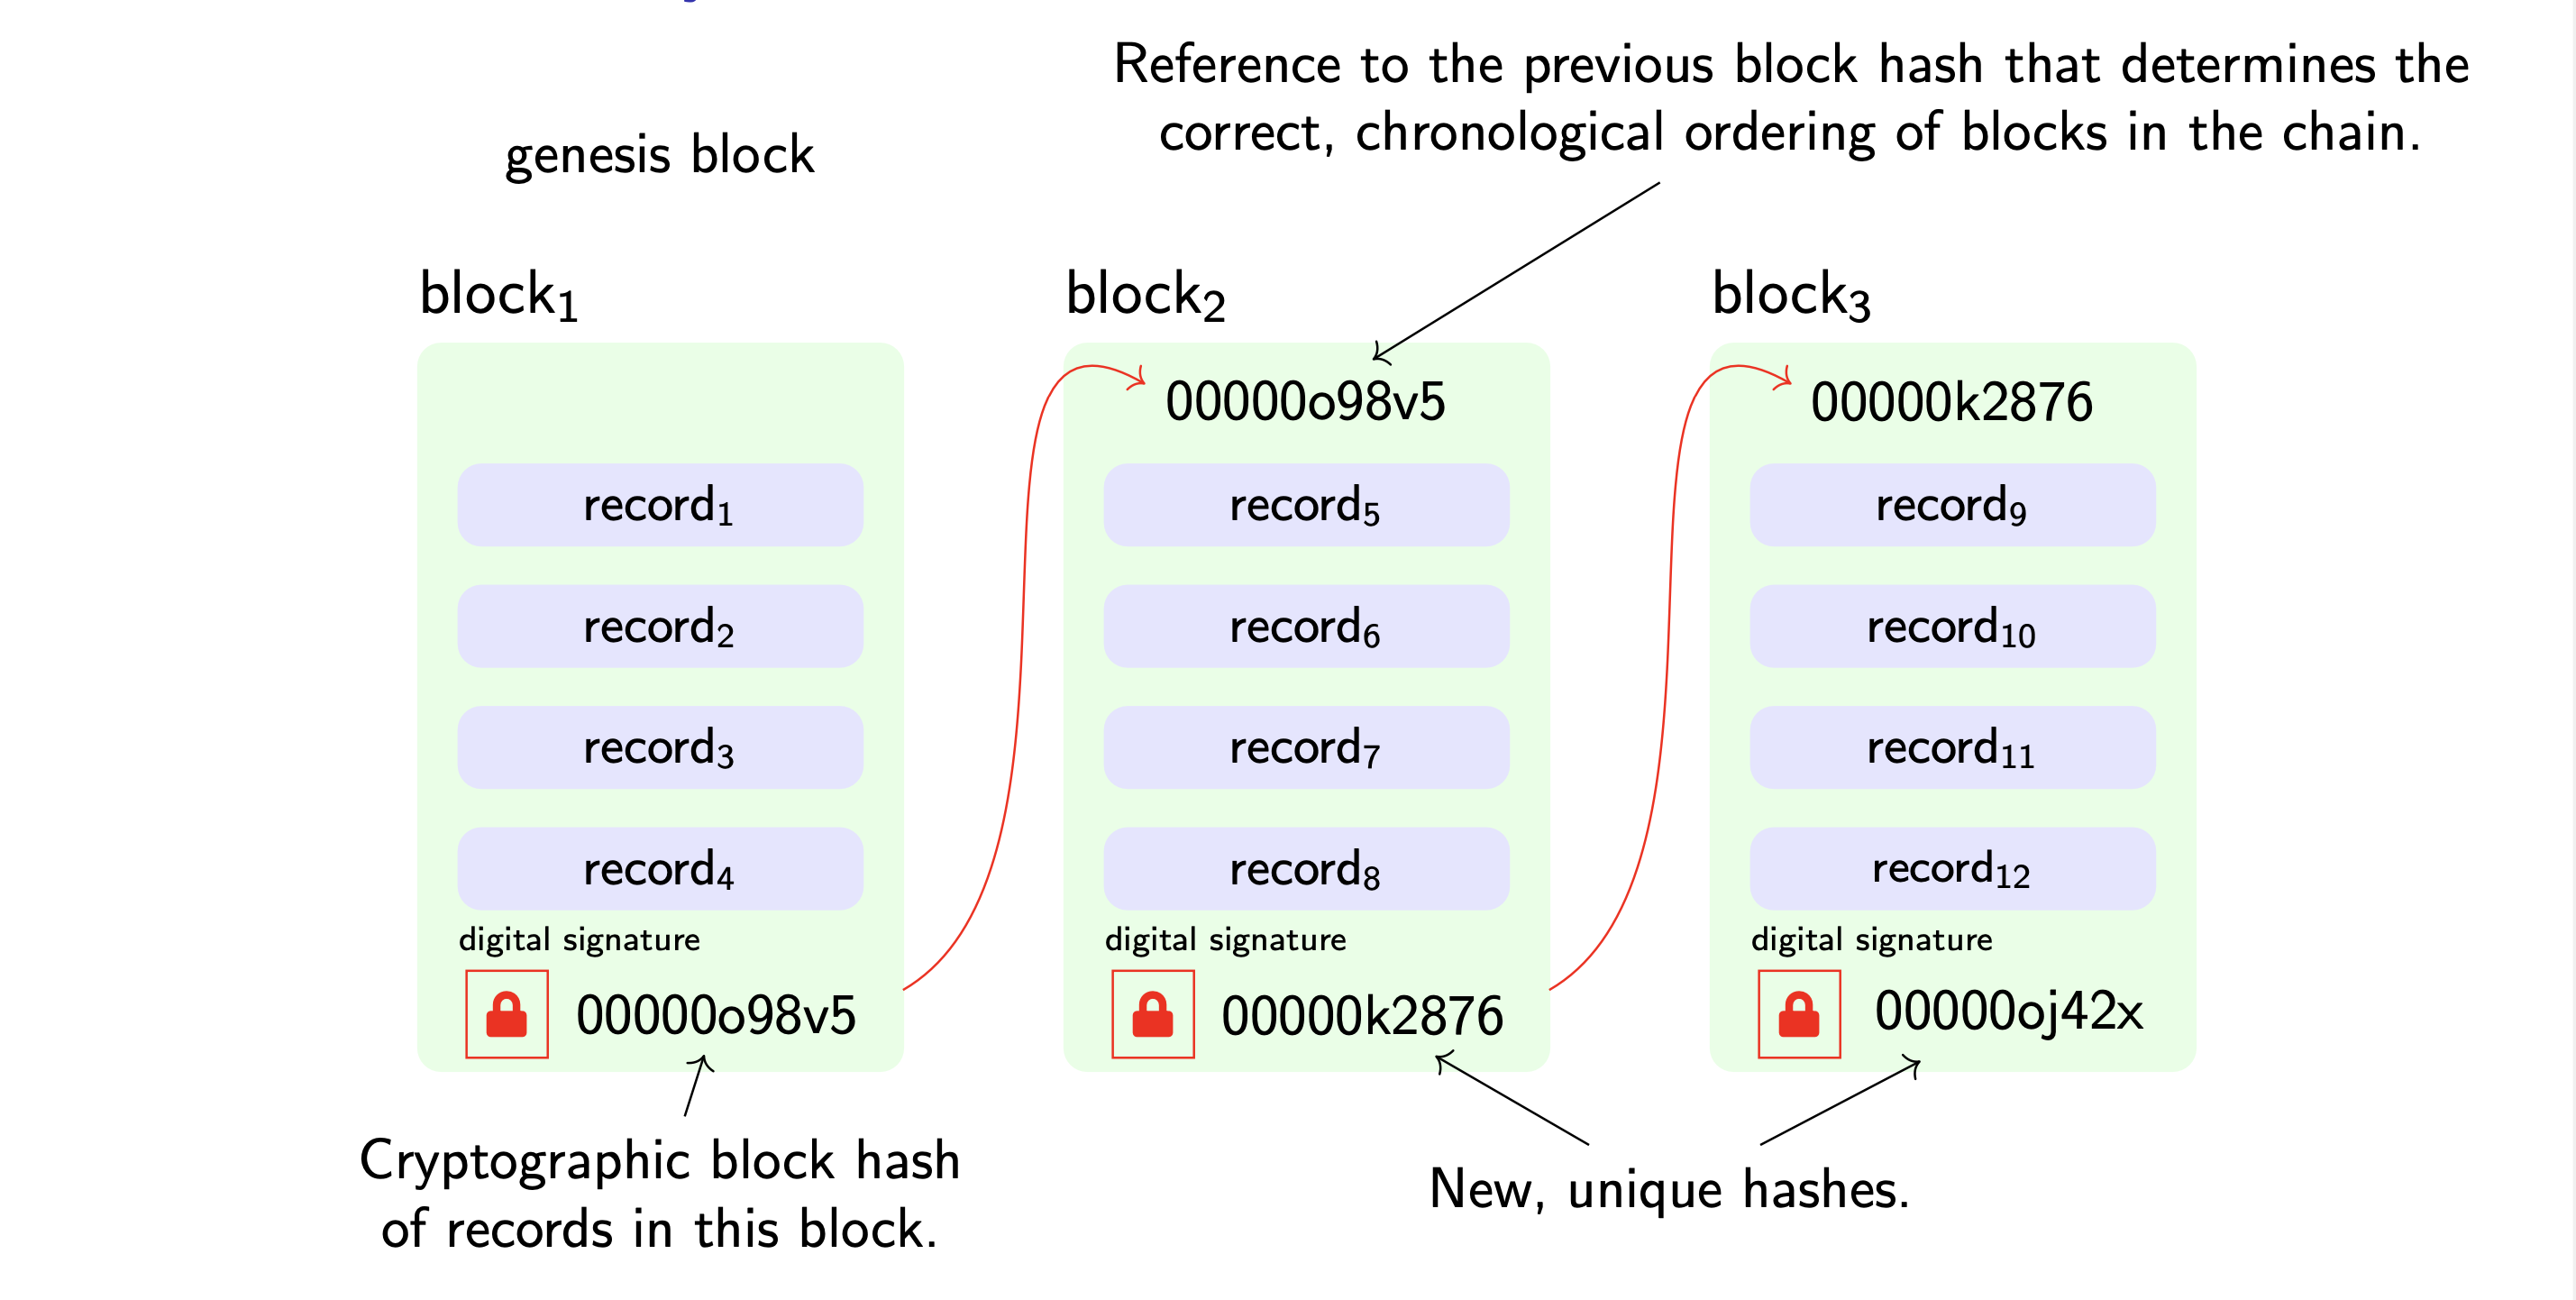
\includegraphics[scale = 0.25]{Screenshot 2025-01-27 at 7.03.18 PM.png}
\end{center}
    
\end{frame}

\begin{frame}{A Centralized Blockchain}

Say that I, JPH, own and operate a private server which records a Blockchain. I don't know the users' private keys, but I control everything that is written on the blockchain. Can I: \pause 
\begin{itemize}
    \item Create false messages? \pause 
    \bi 
    \m No: I don't have the private keys to create messages that can be verified as true. \pause 
    \ei 
    \item Cancel or revert messages? \pause
    \bi 
    \m Yes: I can refuse to include a new block or roll back the blockchain to a previous state. \pause 
    \ei 
    \item Selectively cancel three messages ago, but not the last two? \pause 
    \bi 
    \m No: the hashes of the last two messages would be wrong if the middle hash is missing. 
    \ei 
\end{itemize}
    
\end{frame}

\begin{frame}{A Centralized Blockchain}

Centralized Blockchains are in fact widely-used: 

\bi 
\m Binance Smart Chain 
\m Coinbase Base 
\m Ripple XRP 
\ei \pause 
When are these better than just a spreadsheet? \pause \\ 
\bi 
\m Often they aren't: Chase, VISA, Zelle, and Federal Reserves are all just spreadsheets at the end of the day \pause 
\m Centralized Blockchains add an extra level of security: create a transaction history that can't be arbitrarily tampered with -- only rolled back entirely or stopped pre-emptively. \pause  
\m That's still a lot of power in the admin's hands! \pause 
\ei 

\textbf{Can we take away even more power from the admin? Can we make a set of rules to agree on a shared history of transactions without needing to trust \ul{anybody}?}

\end{frame}


\subsection{A Decentralized Blockchain}

\begin{frame}{A Decentralized Blockchain}

\begin{itemize}
    \item  A natural, “democratic” rule would be to have multiple admins taking turns adding transactions to the chain \pause 
    \item How do we prevent one admin from just pretending to be multiple admins? \pause 
    \item Needs to be some “cost”/“barrier” to becoming an admin \pause 
    \item Bitcoin solves this through \textbf{proof of work}
\end{itemize}
    
\end{frame}


\begin{frame}
\frametitle{Hash Puzzles}

\bi
\m The amount of computational power in the world is finite!
\m Let's try to \href{https://emn178.github.io/online-tools/sha256.html}{find a number whose SHA256 hash has a 0 at the beginning}\ldots \pause 
\m Why is this a nice puzzle? Like a PhD
\be
\m Hard to do
\m Proves that you did something hard to do \pause 
\ee
\m With puzzle solution in hand, you become the admin!
\m \textbf{Incentives:} solving the puzzle gives you some BTC as a \ul{block reward}
\m \textbf{Consensus:} \ul{everyone works on the longest chain} 
\ei

\end{frame}



\begin{frame}{How to Prevent Doublespending?}
    
\bi
\m I may want to spend some money to buy a coffee, then ``unspend'' it (but keep my coffee!)
\m Can't just selectively delete the transaction from history (why?)\pause 
\bi
\m Hashes verify integrity of history!
\ei
\m But\ldots could go back in time, then create a parallel universe (a fork in the chain) where I never spent the money 
\bi
\m This would be called a \ul{doublespend}
\ei
\ei

\end{frame}

\begin{frame}
\frametitle{Turning Back Time\ldots}

\bi
\m Anyone can try, since anyone can try to mine and become admin
\m When would I succeed? \pause
\bi
\m Because everyone uses the \textbf{longest chain}, I must be able to hash faster than \textbf{everyone else combined}
\m Control 51\% of the computing power in the Bitcoin ecosystem!
\ei
\m For more details, see \href{https://cs251.stanford.edu/lectures/lecture5.pdf}{Stanford CS251 slides}
\ei

\end{frame}

\begin{frame}{Welcome! Today is Wednesday 9/17}

Your first homework is due on Canvas by the \textbf{start of class} on Monday. 

\vfill 
Also for \textbf{Monday:} read the Ethereum Whitepaper: 

\begin{center}
    \hyperlink{https://ethereum.org/whitepaper/}{https://ethereum.org/whitepaper/}
\end{center}

Guide your reading by thinking about the following questions: 
\begin{itemize}
    \item What is a Smart Contract? 
    \item How do fees in Ethereum differ from fees in Bitcoin? 
    \item Why do Turing-complete smart contracts require a different fee structure? 
\end{itemize}

    
\end{frame}

\begin{frame}{In the News: Google's Agent Payment Protocol}

\begin{center}
    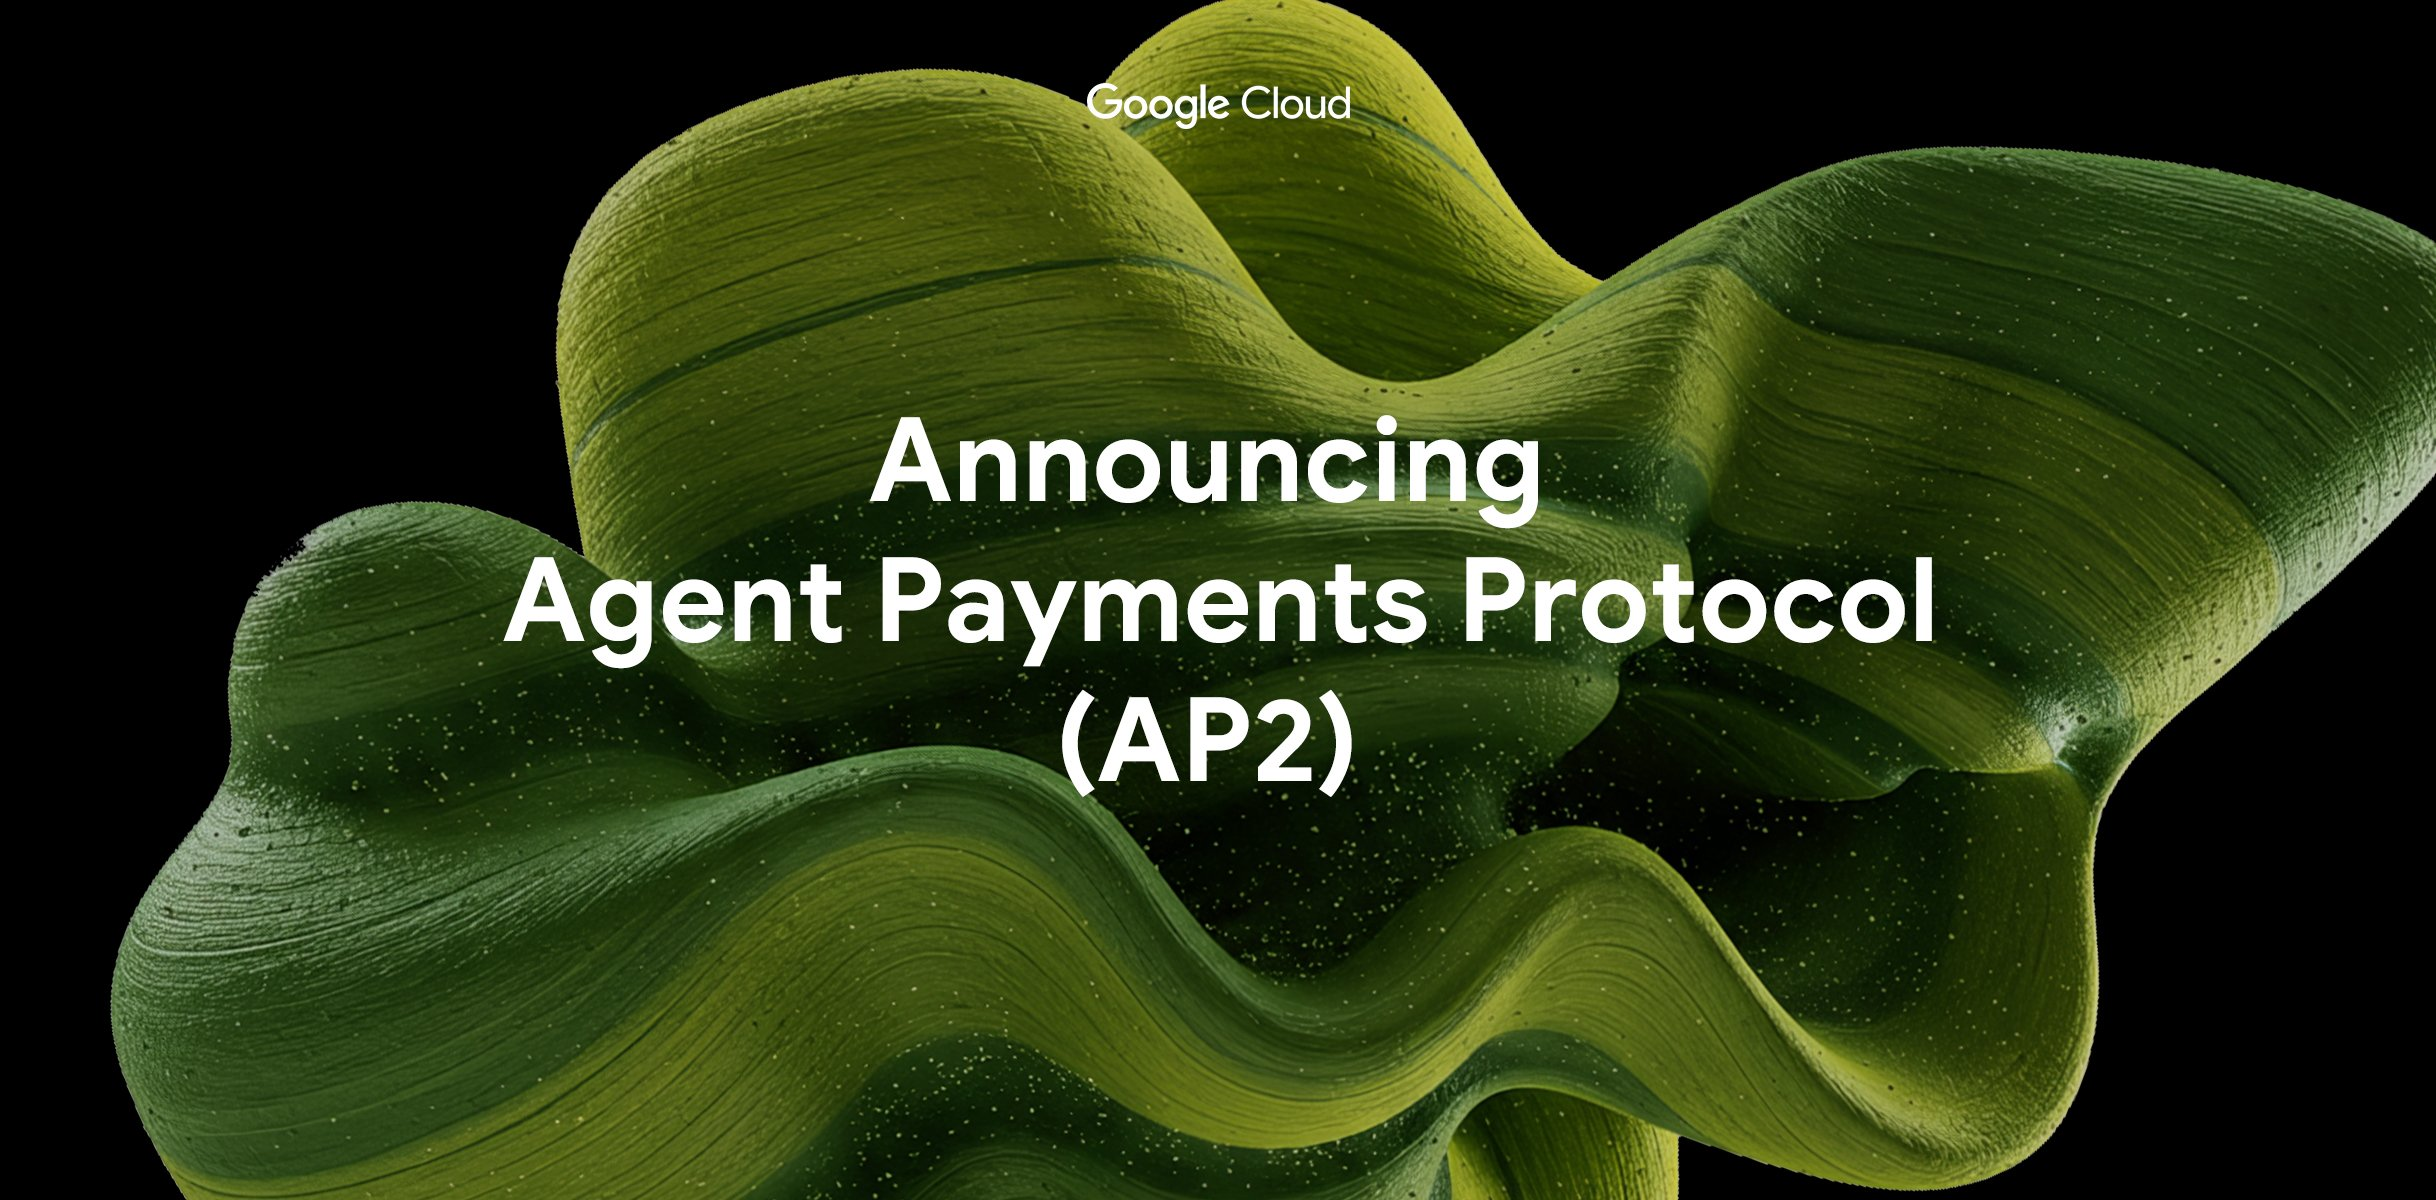
\includegraphics[width = \textwidth]{AP2.jpg}
\end{center}    
    
\end{frame}

\begin{frame}{In the News: Google's Agent Payment Protocol}
    \begin{center}
    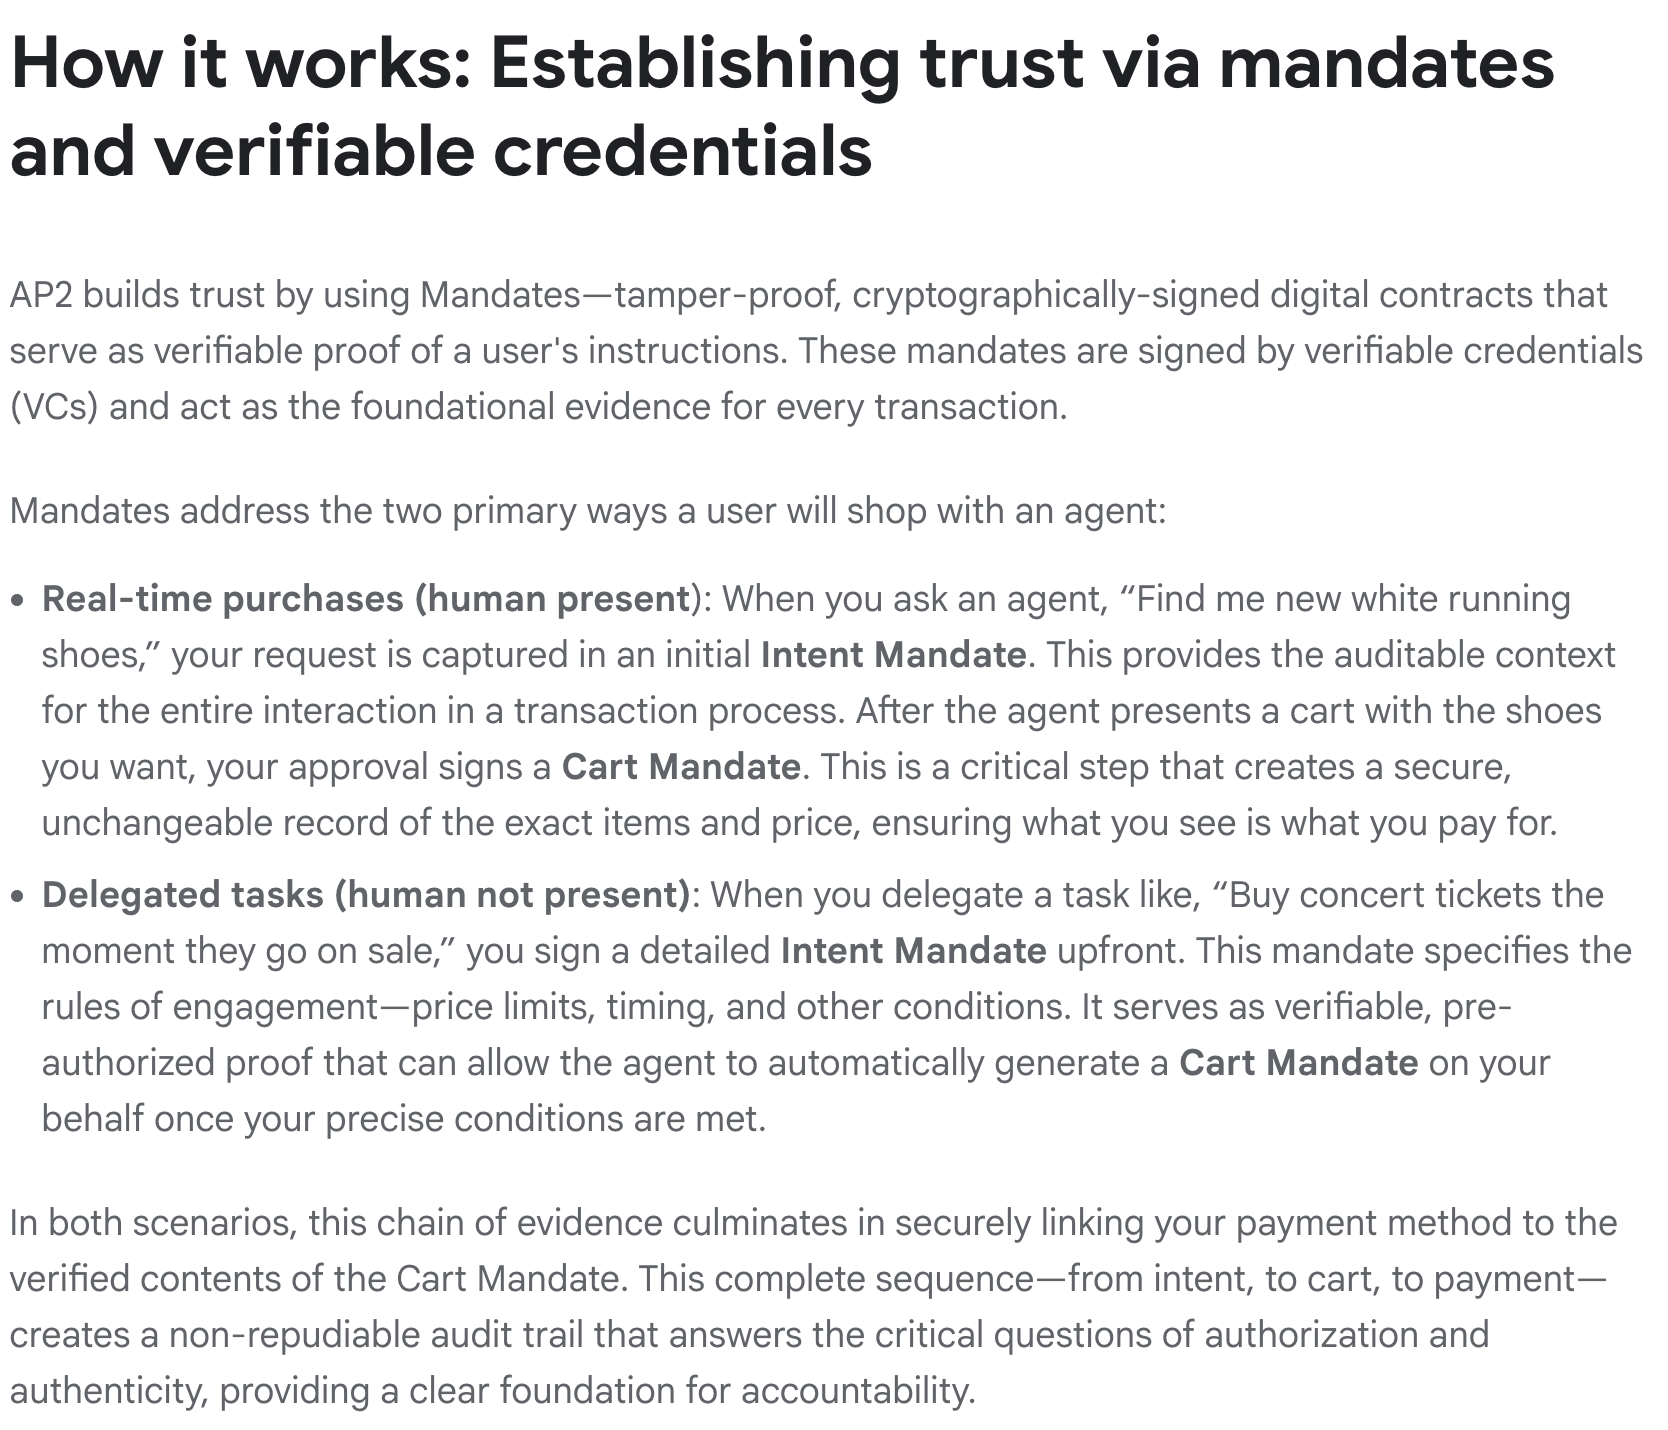
\includegraphics[height = .9\textheight]{A2p2.png}
\end{center}
\end{frame}

\subsection{Mining}

\subsection{Some Basic Game Theory}

\begin{frame}
\frametitle{The Money Pot Game}

\bi
\m Two options:
\be
\m Get \$1 for sure
\m Fight for a \$10 pot, which is equally divided between everyone who picks this option
\ee \pause
\m Which do you pick?
\ei

\end{frame}

\begin{frame}
\frametitle{The Money Pot Game}

\bi
\m What is going on?
\bi
\m Everyone wants the money pot
\m But the more people take the money pot, the less money there is for everyone
\m In ``Nash equilibrium'', the money pot becomes no better than the ``outside option''
\ei \pause
\m Similar settings: what's the equilibrium condition?
\bi
\m Firms competing for profits? \pause
\m Going to the beach on a sunny day? \pause
\m Getting a table for Brunch on Sunday at 12pm? \pause
\ei
\m ``Equilibrium'' behavior is easy to predict in such settings
\bi
\m In equilibrium, the ``good'' deal is so crowded that it becomes just as bad as the ``bad'' deal
\ei \pause
\m Game theory language: call these \ul{congestion games}, or \ul{wars of attrition}, or \ul{tragedy of the commons}
\ei

\end{frame}

\subsection{Difficulty Adjustments}

\begin{frame}
\frametitle{BTC mining}

\bi
\m Suppose mining a block pays 0.001 BTC
\m Suppose mining block costs \$60 in electricity
\bi
\m If BTC price $>\$60k$, everyone mines; blocks produced quickly
\m If BTC price $<\$60k$, nobody mines; tx's aren't included and the blockchain stops working!
\ei
\m The fact that mining rate depends on BTC vs electricity price is not desirable\ldots
\m Solution: use \ul{difficulty adjustment} to maintain constant block production rate
\ei

\end{frame}

\begin{frame}
\frametitle{BTC Difficulty Adjustment}

\bi
\m Blocks should be produced every 10 minutes
\m Every 2016 blocks (approx 14 days), Bitcoin considers average block production rate, and\ldots
\bi
\m Increases/decreases hash problem difficulty, if block production is too fast/slow
\ei
\m What determines how fast blocks are produced, fixing hash rate? \pause
\bi
\m How many people (that is, how much electricity) is devoted to mining
\ei \pause
\m What determines how many people mine?
\bi
\m How profitable mining is, that is, how high BTC price is, vs electricity price
\ei
\ei

\end{frame}


\begin{frame}
\frametitle{BTC: Equilibrium Condition}
What happens to mining when BTC price goes up?
\bi \pause
\m More people try to mine
\m Difficulty goes up; so electricity to mine a BTC increases
\m $\implies$ profit per \$ of electricity spent doesn't change
\ei \pause
\textbf{Prediction:} difficulty should increase with BTC price

\end{frame}

\begin{frame}
\frametitle{Difficulty vs BTC price}

\begin{center}
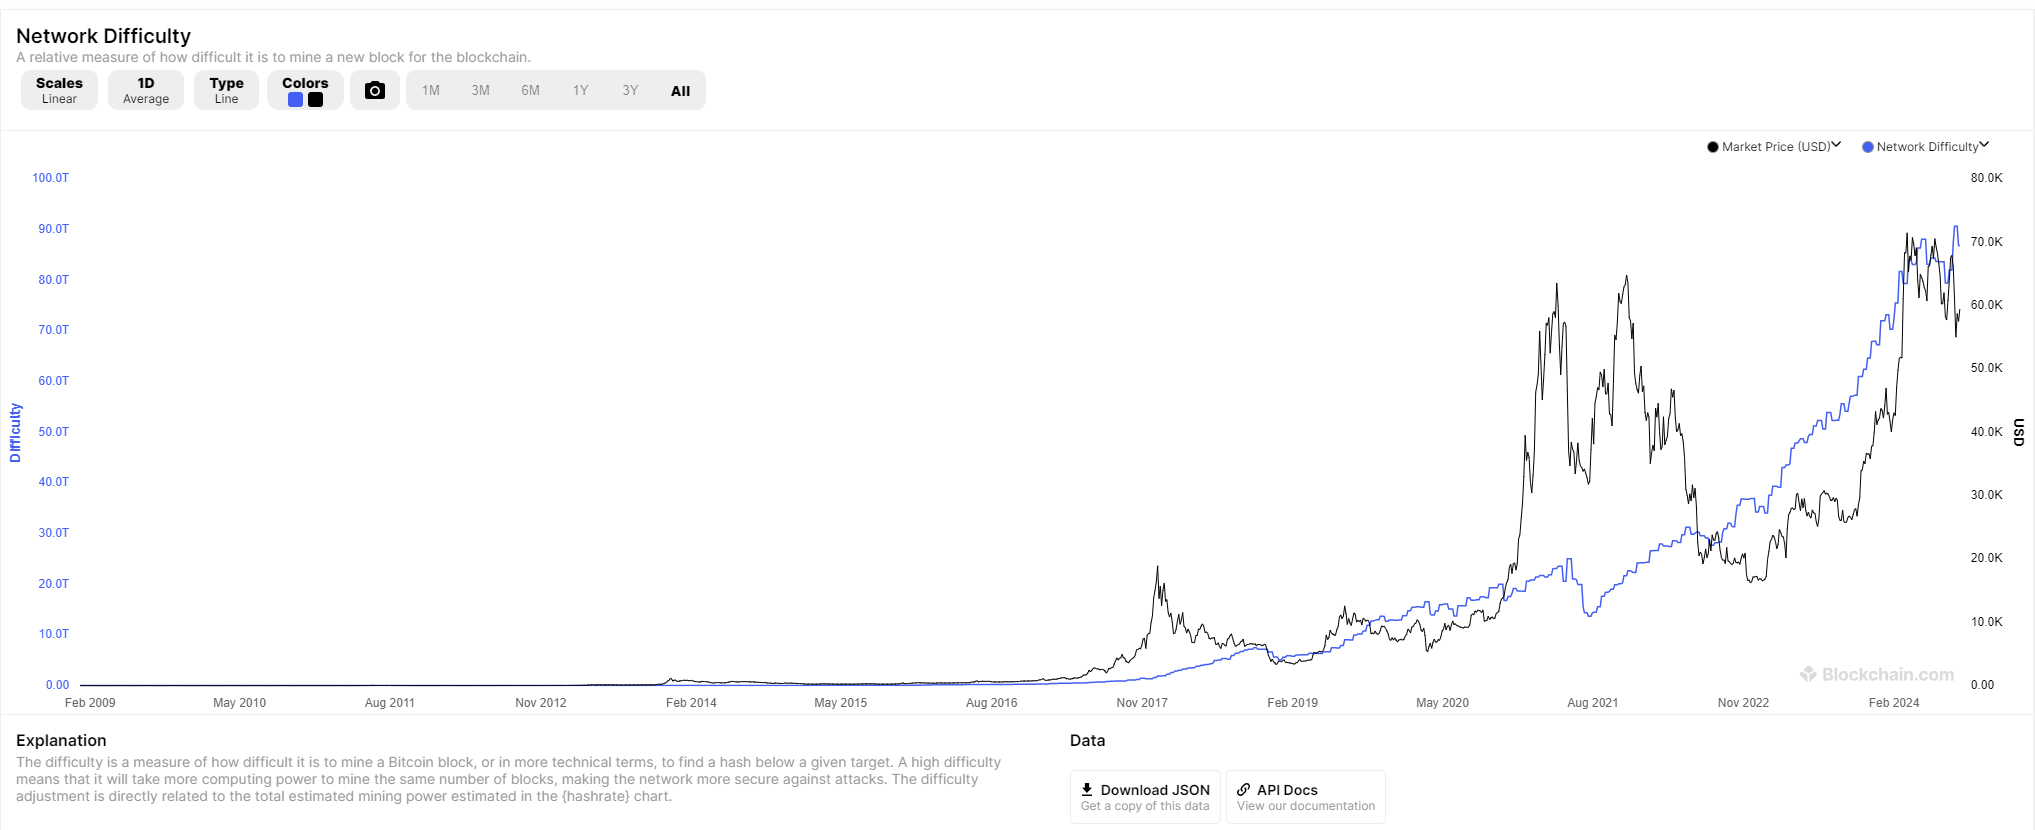
\includegraphics[width = \textwidth]{pics/difficulty.png}
\end{center}


\scriptsize
Source: \href{https://www.blockchain.com/explorer/charts/difficulty}{Blockchain.com}

\end{frame}

\begin{frame}
\frametitle{Energy Prices\ldots}

\begin{center}
	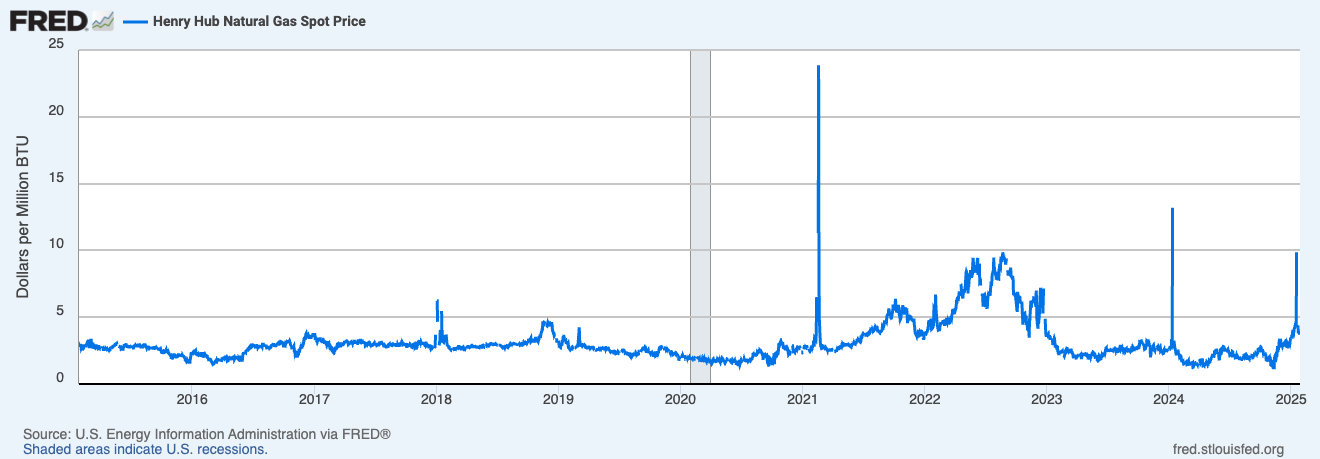
\includegraphics[width = \textwidth]{fredgraph.png}
\end{center}

\scriptsize
Source: \href{https://fred.stlouisfed.org/series/DHHNGSP}{FRED} \\ \pause 
A \textbf{BTU} is a ``British Thermal Unit'', the energy required to heat a pound of water by 1 degree Fahrenheit (about one match) 

\end{frame}



%Source: \href{https://data.hashrateindex.com/chart/asic-price-index}{Hashrate Index}


%Circle plot: money, electricity, hashes, BTC, money


\begin{frame}
\frametitle{Technological Improvement}

\begin{center}
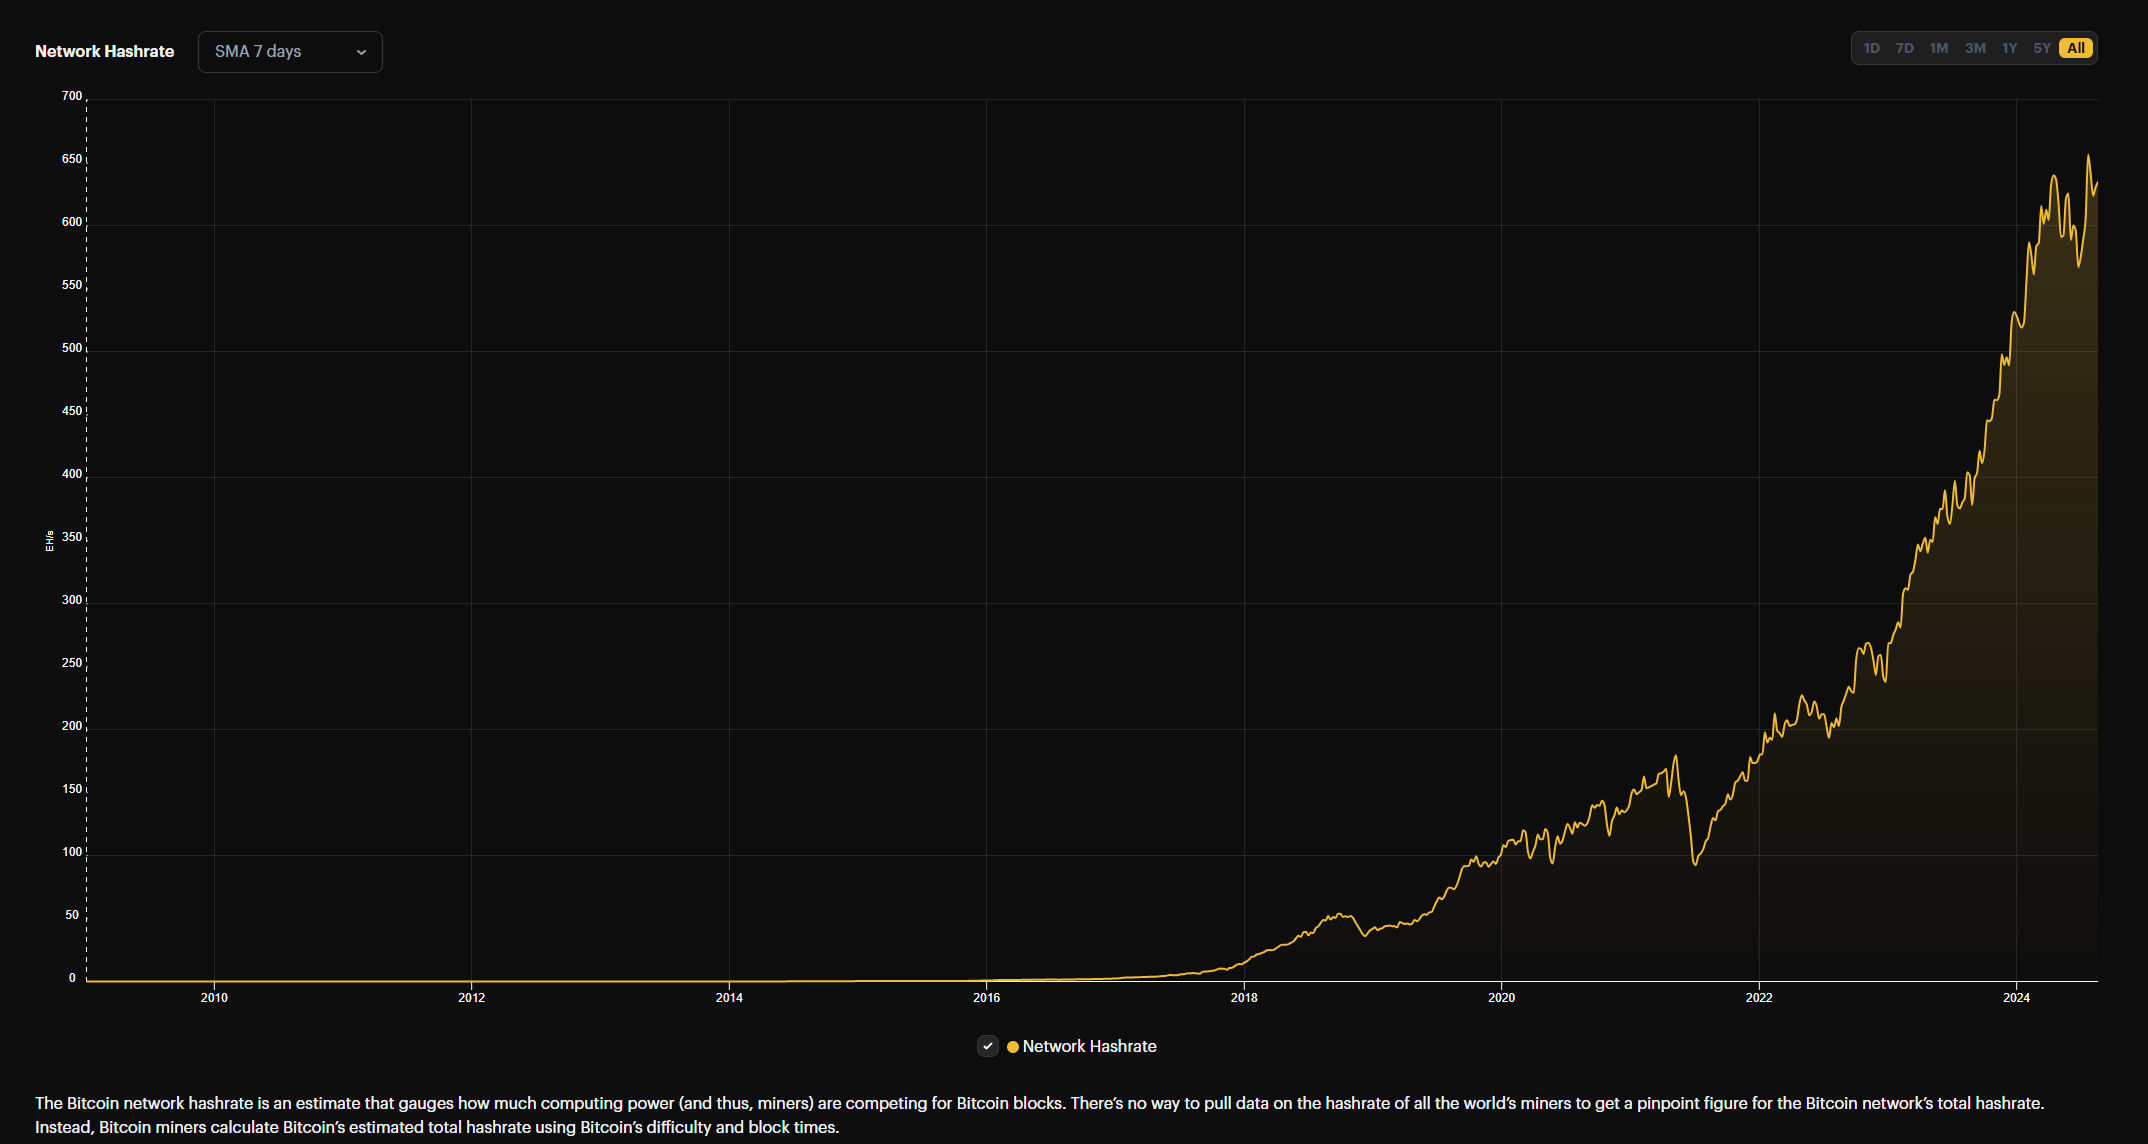
\includegraphics[width = 0.65\textwidth]{pics/hashrate.png}
\end{center}

\bi
\m 842 Exahashes/s = 842 billion billion hashes a second!
\m Each living person in the world could shake each other living person's hand 10 times, every second!
\m $\sim1\%$ of global energy consumption\ldots
\ei

\scriptsize
Source: \href{https://data.hashrateindex.com/chart/bitcoin-network-hashrate}{Hashrate Index}

\end{frame}

\begin{frame}
\frametitle{Back-of-Envelope Calculation}

As of 2024,
\bi
\m 164,250 BTC mined per year, worth around \$8bil
\bi
\m In theory, what should total mining costs be?
\ei \pause
\m Back of envelope calculation\ldots
\bi
\m World electricity consumption approx 25,000TWh; BTC mining around 0.5\%, so 125TWh 
\m At US price \$0.12/kWh, this is approx \$15bil!
\m (a kWh (kilo-Watt-hour) is 3,412 BTUs) 
\ei
\m Electricity is probably somewhat cheaper, getting us close to \$8bil \pause
\m Will this decrease as technology improves?
\bi
\m No! Problem difficulty will just adjust\ldots
\ei
\m What if BTC price falls?
\ei

\end{frame}

\begin{frame}
\frametitle{BTC Halving}

\bi
\m Approximately every 4 years, issuance of BTC drops by half
\m Last halving: April 2024, now 3.125 BTC per block
\m Does this affect block production rate?
\bi
\m No, difficulty adjustment
\ei \pause
\m Also implies there will only ever be 21 million BTC in existence!
\bi 
\m By approximately 2140, the block reward will drop to less than the smallest unit of bitcoin ($1/10^8$) and become equal to zero. 
\m Difficulty adjustment ensures that block production rate is approximately constant 
\ei 
\ei

\end{frame}

\begin{frame}
	\frametitle{Why 21 Million?}
	
	\footnotesize
	
	\href{https://mmalmi.github.io/satoshi/}{Satoshi:} ``My choice for the number of coins and distribution schedule was an 
	educated guess.  It was a difficult choice, because once the network is 
	going it's locked in and we're stuck with it.  I wanted to pick 
	something that would make prices similar to existing currencies, but 
	without knowing the future, that's very hard.  I ended up picking 
	something in the middle.  If Bitcoin remains a small niche, it'll be 
	worth less per unit than existing currencies.  If you imagine it being 
	used for some fraction of world commerce, then there's only going to be 
	21 million coins for the whole world, so it would be worth much more per 
	unit.  Values are 64-bit integers with 8 decimal places, so 1 coin is 
	represented internally as 100000000.  There's plenty of granularity if 
	typical prices become small.  For example, if 0.001 is worth 1 Euro, 
	then it might be easier to change where the decimal point is displayed, 
	so if you had 1 Bitcoin it's now displayed as 1000, and 0.001 is 
	displayed as 1.''
	
\end{frame}



\begin{frame}{Transaction Fees}

\bi 
\m Block rewards are not the only incentive to process transactions: miners also charge \ul{transaction fees} to include a transaction in their blocks. \pause 
\m Transaction fees are quoted in ``sat/vB'', or ``Satoshis per virtual Byte" 
\bi 
\m A \ul{Satoshi} is $1/10^8$ BTC, the smallest unit that can be transacted \pause 
\m The \ul{Size} of the transaction depends mostly on its format. \href{https://mempool.space/docs/faq}{The current most efficient format for submitting transactions was created in 2017.} \pause 
\ei
\m Miners prioritize including transactions that offer higher fee rates 
\m As of 2/4/25, the going rate to complete your transaction within 30 minutes is 3 sat/vB, or	$\$0.42$ for an average transaction \pause 
\m A \textbf{``mempool''} is a pool of transactions waiting to be added to the bitcoin blockchain 
\ei 

Explore mempools at \hyperlink{https://mempool.space/}{https://mempool.space/}
    
\end{frame}


\begin{frame}
	\frametitle{Transaction Fees as \% of Block Revenue}
	
	\begin{center}
		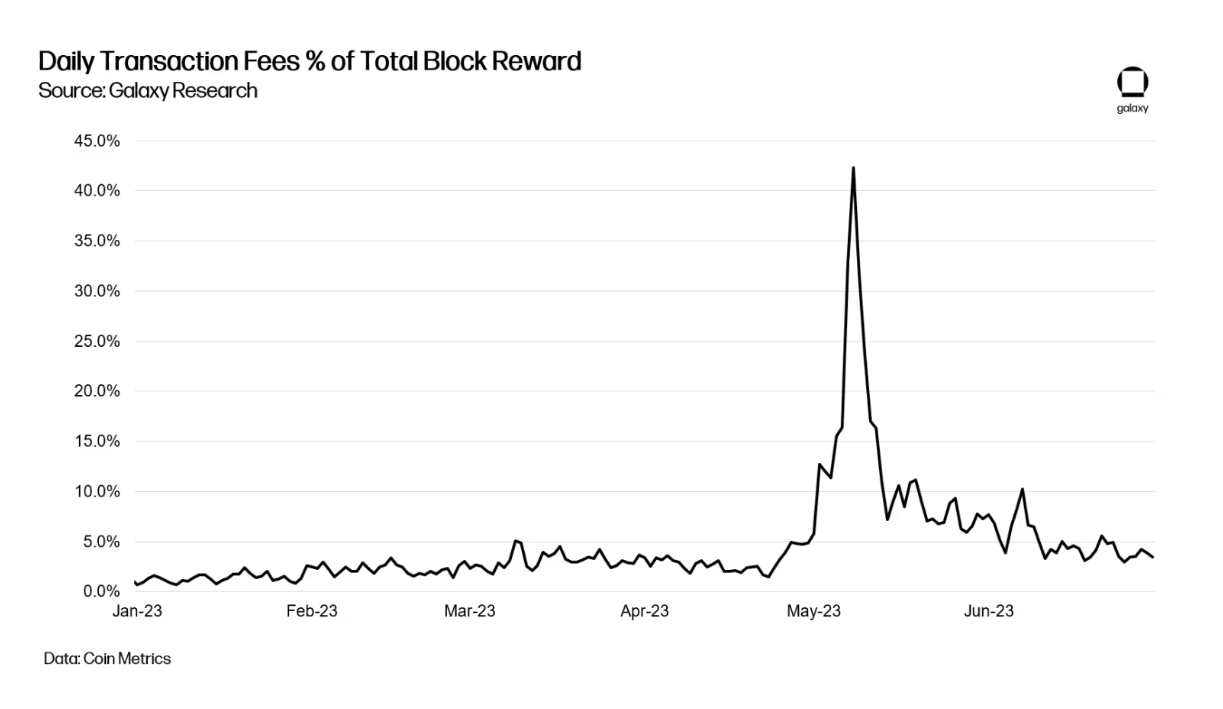
\includegraphics[width = 0.8\textwidth]{pics/txfeespct.png}
	\end{center}
	
	Source: \href{https://www.galaxy.com/insights/research/2023-mid-year-mining/}{Galaxy}
	
\end{frame}

\begin{frame}
\frametitle{Incentives}

\bi
\m A centralized authority can ``censor'', i.e. not include tx's
\m Decentralization and competition ``ensure'' performance
\bi
\m If you don't include my tx, the next miner will
\m Even if the US bans US miners from including tx's, someone else will include them
\ei
\m More or less works for just transacting \pause
\m Incentives not that strong: tx fees $<10\%$ of mining revenues
\bi
\m But, it's free \$\$!
\ei
\ei

\end{frame}


\begin{frame}
\frametitle{Further Reading on Mining Industry}

\bi
\m Galaxy digital \href{https://www.galaxy.com/insights/research/2023-mid-year-mining/}{2023} and \href{https://www.galaxy.com/insights/research/2024-mid-year-mining/}{2024}
\m Cool \href{https://zhiguohe.net/wp-content/uploads/2023/12/10914-hhaa040.pdf}{paper} on mining pools
\ei

\end{frame}


\section{Bitcoin}

\subsection{History}

\begin{frame}
\frametitle{Satoshi Nakamoto}

\bi
\m Started sending emails about Bitcoin August 2008
\m Oct 2008: Bitcoin \href{https://bitcoin.org/bitcoin.pdf}{white paper}, code released
\m January 9: first block mined!
\bi
\m ``The Times 03/Jan/2009 Chancellor on brink of second bailout for banks''
\ei
\m May 22, 2010: Laszlo Hanyecz bought two Papa John's pizzas for 10,000 BTC, now worth \$600mil USD!
\m Quickly became popular among black markets, \href{https://en.wikipedia.org/wiki/Silk_Road_(marketplace)}{Silk Road}\ldots
\m Founder Ross Ulbricht was recently pardoned by Trump 
\ei
	
\end{frame}

\begin{frame}
\frametitle{Prizes for a Starcraft Tournament in 2011}

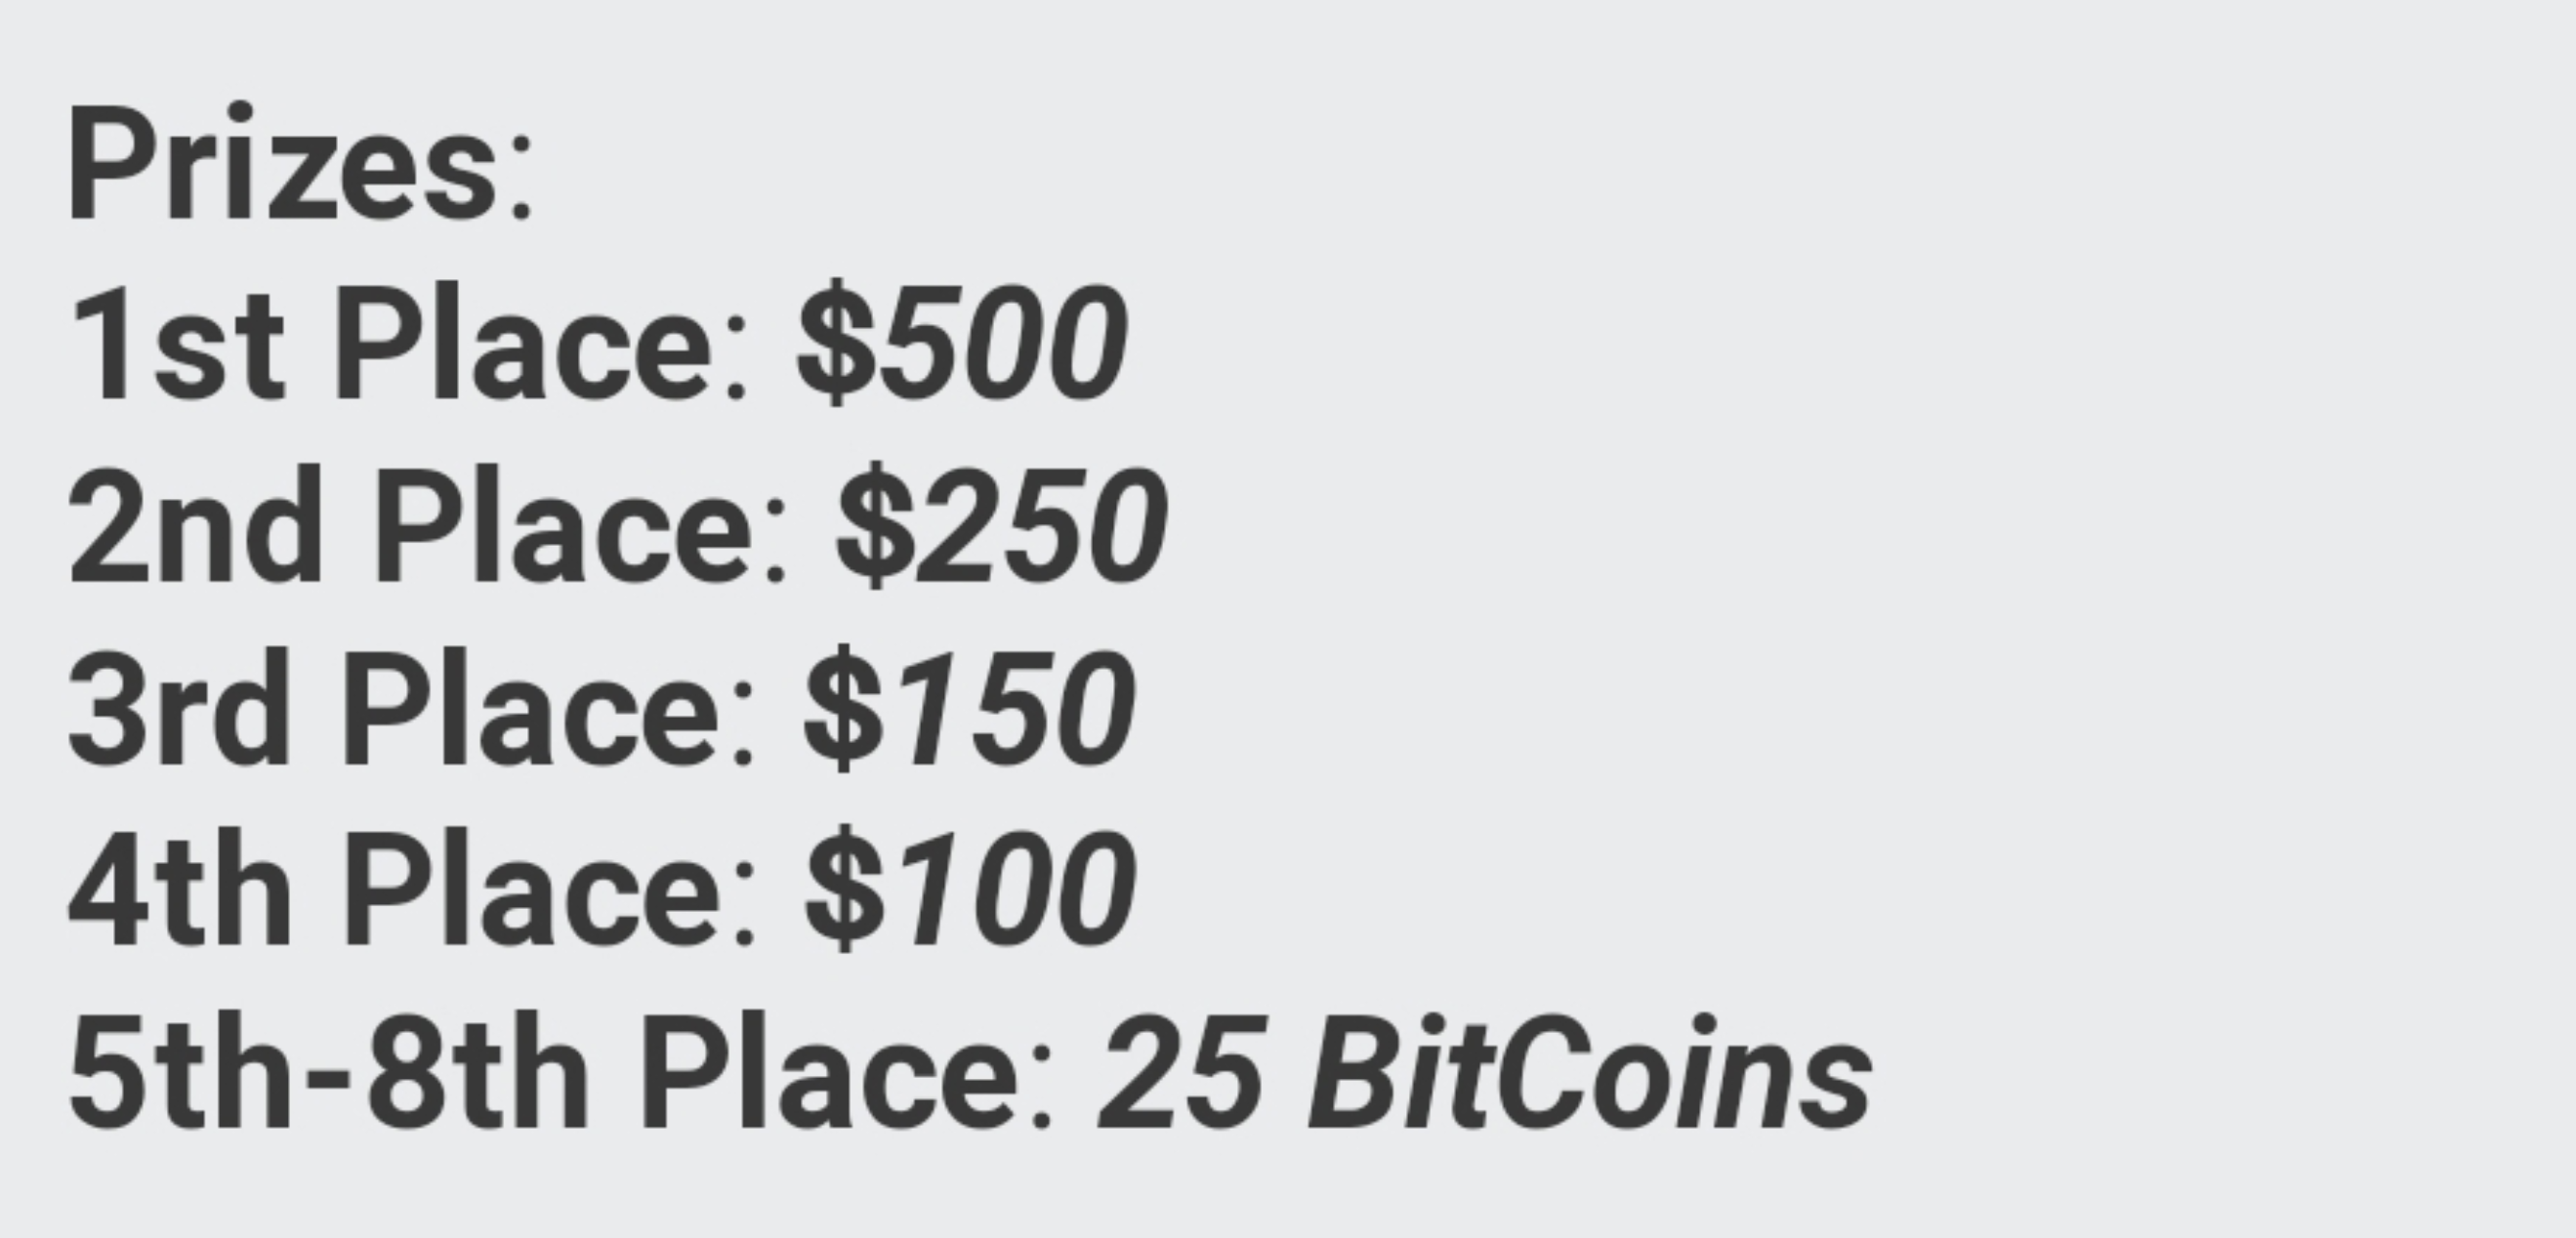
\includegraphics[height = 0.8\textheight]{Screenshot 2025-01-28 at 3.03.46 PM.png}
    
\end{frame}



\begin{frame}
\frametitle{Bitcoin Prices}

\begin{center}
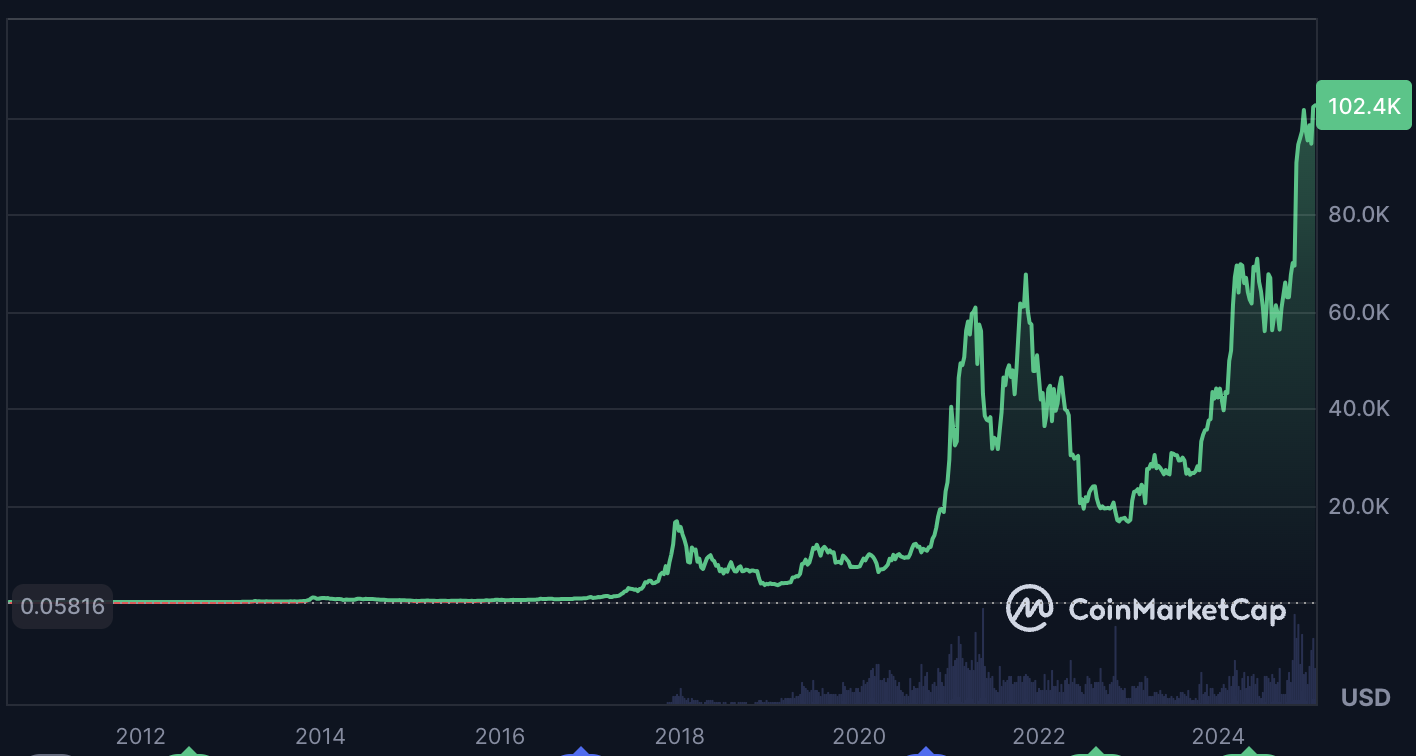
\includegraphics[width = .8\textwidth]{Screenshot 2025-01-28 at 3.02.23 PM.png}
\end{center}

\scriptsize
Source: \href{https://coinmarketcap.com/currencies/bitcoin/}{CoinMarketCap}

\end{frame}

\subsection{Technical Details}

\begin{frame}
\frametitle{Each BTC Block is a Merkle Tree of Transactions!}

\begin{center}
	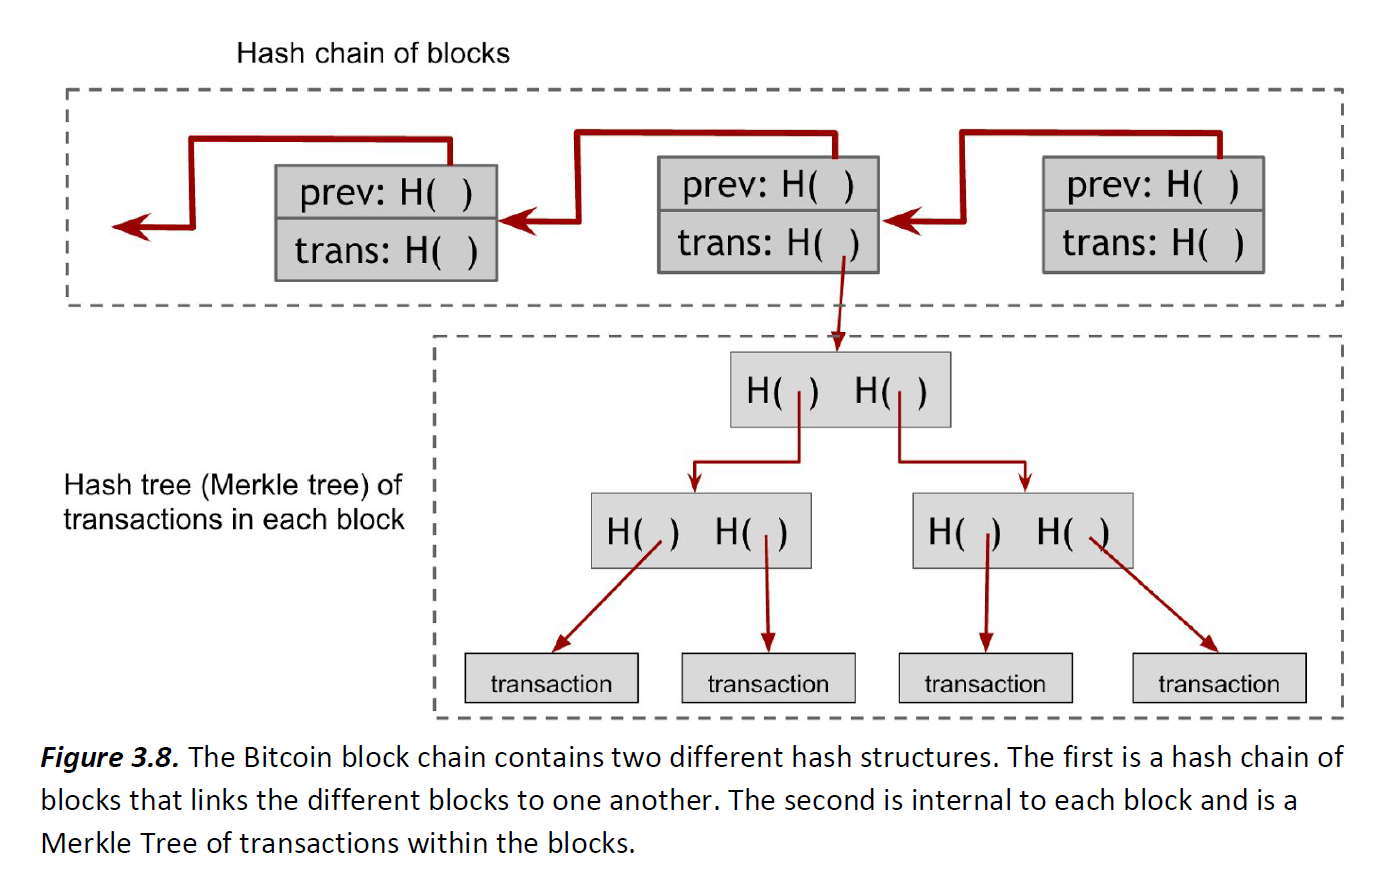
\includegraphics[width = 0.65\textwidth]{pics/blockchain_book.png}
\end{center}

\bi
\m Valid block headers' hashes start with a big number of 0's (mining puzzle)
\ei

\vspace{2ex}

\scriptsize

Source: \href{https://d28rh4a8wq0iu5.cloudfront.net/bitcointech/readings/princeton_bitcoin_book.pdf?a=1}{NBFMG}, fig. 3.8

\end{frame}

\begin{frame}
\frametitle{Mining, in Practice}

\bi
\m Miners connected to each other in a network
\m If you find a valid block, tell all other miners about it
\bi
\m They'll then mine the next block, based on yours
\ei
\m If you solved the hash puzzle, why can't I just steal your solution? \pause
\bi
\m My address is hashed into the block header 
\ei\pause
\m Why wouldn't I try to re-mine your block? \pause
\bi
\m Consensus: if everyone else uses ``longest chain'', I do better by accepting your win, and trying to mine the next block
\ei
\ei

\end{frame}

\begin{frame}
\frametitle{The Power of Consensus}

\bi
\m Notice that all properties depend on everyone ``following the rules''\ldots
\bi
\m If your block:
\bi
\m Doesn't hash to enough 0's, or
\m Steals \$\$, or
\m Includes invalid tx's, etc.
\ei
\m Others won't build on it, so others won't build on others not building on it, 
\m So you won't get mining reward
\ei
\m At some level, maybe the simplicity of the rules, plus the decentralization of mining, provides security?
\bi
\m By default, miners will pick the simplest possible path
\ei
\ei

\end{frame}

\begin{frame}
\frametitle{Transacting, in Practice}

\bi
\m If I want to send, sign a tx, and tell all the miners about it \pause
\bi
\m Pile of valid signed, but not-yet in chain, tx's floating around waiting to be included by miners called the \textbf{mempool}
\ei \pause
\m Why can't miner steal my \$? \pause
\bi
\m Tx specifies signature and receiver; miner can only include tx
\ei
\m What if miner doesn't want to include me? \pause
\bi
\m Someone else will, and take the tx fee\ldots
\m \ldots And miner eventually has to accept my tx as valid, or ``fork'' whole network (since hash pointers break)
\ei \pause
\m What if I try to spend twice? \pause
\bi
\m One tx is ``invalid'': doesn't obey the rules, since old tx output already spent
\m Remember, though; everything is ultimately due to consensus among miners, that ``longest block of valid chains'' is the legitimate blockchain
\ei
\ei

\end{frame}

\subsection{User Experiences}

\begin{frame}
\frametitle{Fees and Times}

\bi
\m Fees: a few cents to a few USD
\bi
\m Doesn't depend on tx size 
\ei
\m Time: roughly 1hr
\bi
\m Most services wait a few blocks (why?) \pause
\m Tx's deeper down the blockchain are more ``final'' (harder to ``doublespend'')
\ei
\m Long confirmation times a little awkward for ``merchant'' tx's
\ei

\end{frame}

\begin{frame}
\frametitle{User Experience}

\bi
\m In practice, private keys held using ``wallet'' software or hardware
\bi
\m Software: Exodus, Electrum, MetaMask\ldots
\m Hardware: Ledger, Trezor\ldots
\m Some mobile app wallets, which I'm not familiar with
\m I use MetaMask 
\ei \pause
\m In theory, no credit risk -- you're holding your own BTC!
\bi
\m As long as internet + Bitcoin exists, you can use your BTC!
\ei
\ei

\end{frame}

\begin{frame}
\frametitle{Don't Lose Your Keys\ldots}

\begin{center}
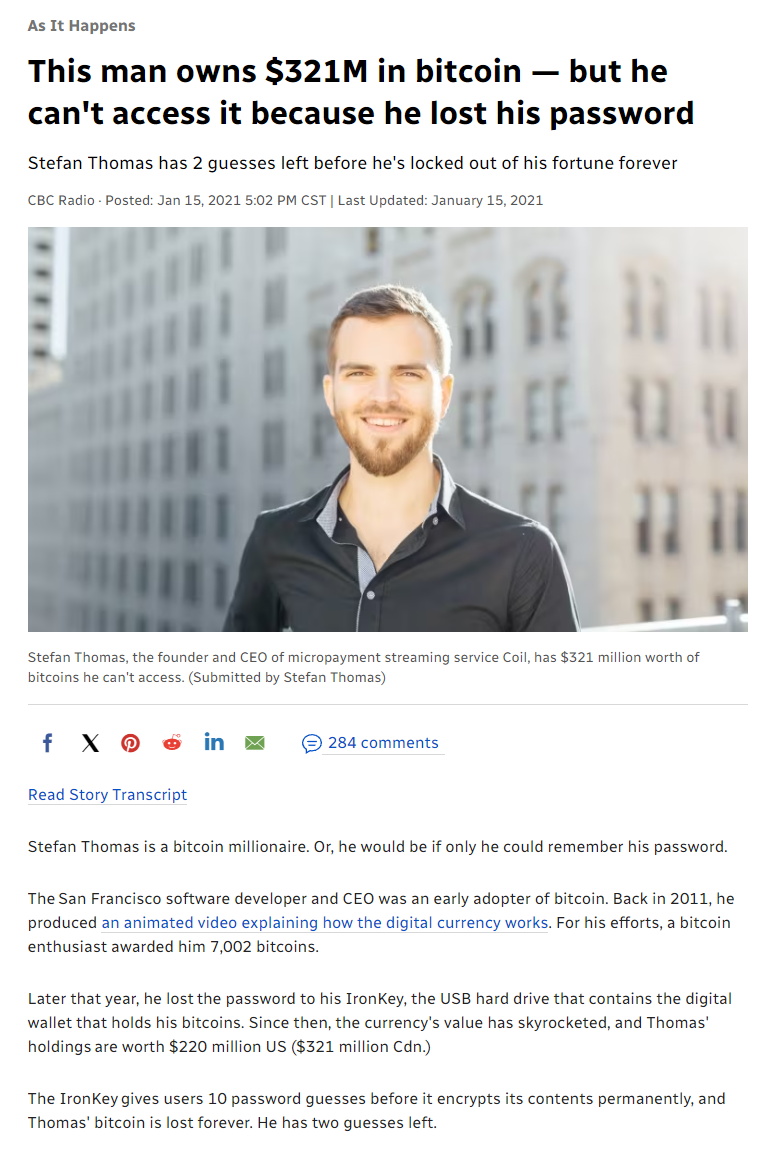
\includegraphics[width = 0.5\textwidth]{pics/lostkeys.png}
\end{center}

\end{frame}

\begin{frame}
\frametitle{Custodial Ownership}

\bi
\m Many don't care about decentralization, censorship-proofness\ldots
\bi
\m But want to buy in case prices go up
\ei
\m More and more ways to buy BTC
\bi
\m Crypto exchanges: Coinbase, Binance\ldots
\m Classic institutions: Paypal, Robinhood\ldots
\ei
\m Recent ETF approvals makes it easier to buy BTC
\m New SEC commissioner Paul Atkins has signaled positivity towards legitimizing crypto investments 
\ei

\textbf{Mentions are not endorsements!}

\end{frame}

\begin{frame}
\frametitle{``Buy the Market''}

The CAPM says buy the market -- and BTC's market cap is now approx 2\% S\&P 500! \pause

\begin{center}
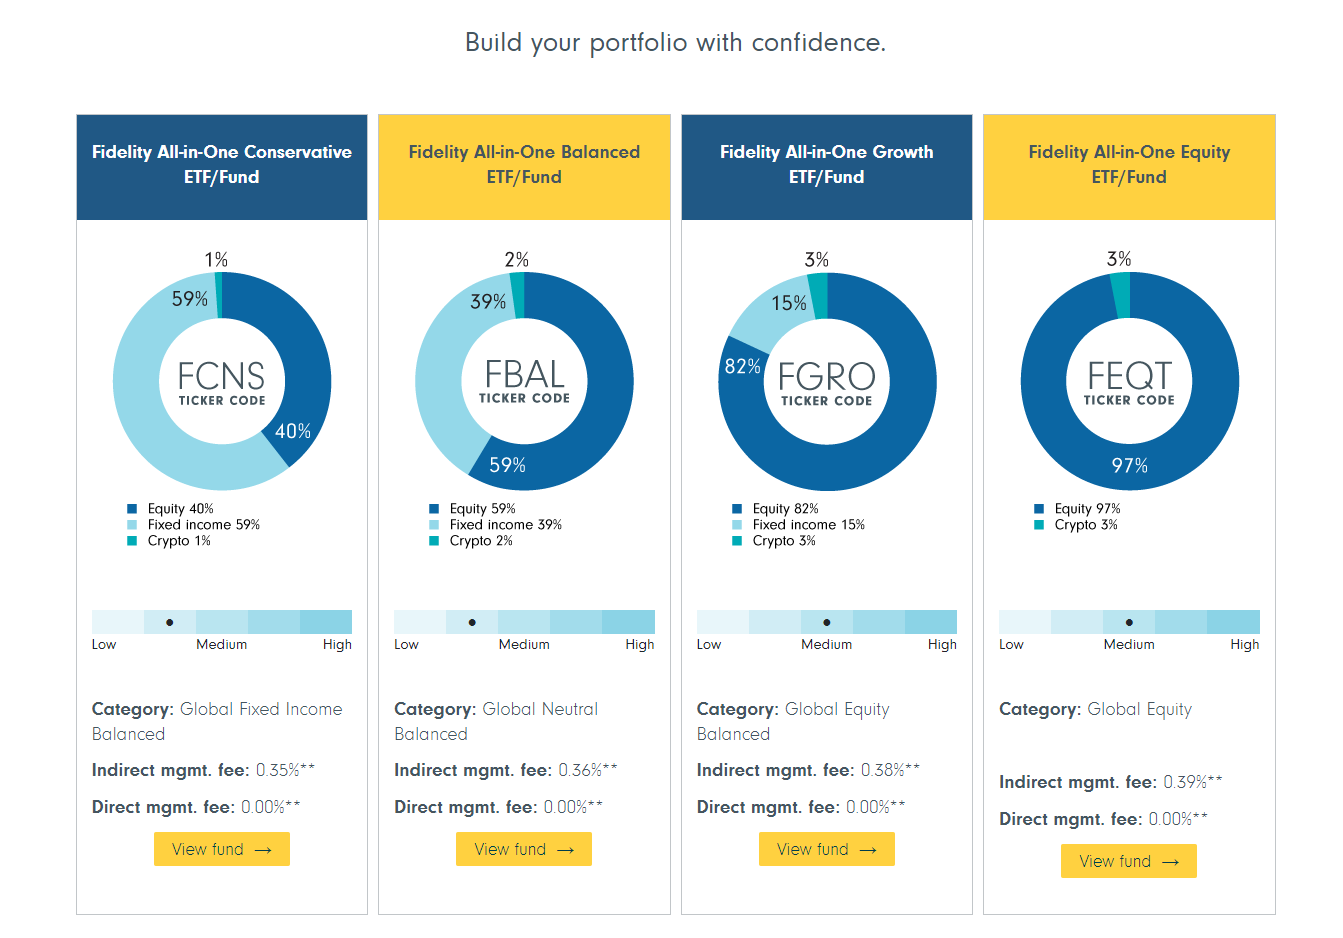
\includegraphics[width = 0.6\textwidth]{pics/Fidelity.png}
\end{center} 

\vspace{2ex}
\scriptsize

Source: \href{https://www.fidelity.ca/en/investments/solutions-portfolios/all-in-one/}{Fidelity Canada}

\end{frame}

\begin{frame}{The ``Market Cap'' Illusion}

\textbf{Market Capitalization} is just units outstanding times unit price 

\bi 
\m Say everyone tried to sell their BTC tomorrow. Would they get that price for it? \pause 
\m Traditional assets (stocks, bonds) generate \textbf{dividends} or \textbf{coupons} 
\bi 
\m If a major owner of a stock worth 2\% of the S\&P500 sold, the supply would be absorbed relatively quickly 
\m Investors are willing to substitute frictionlessly between stocks if one is temporarily undervalued \pause 
\ei 
\m Reports of \$TRUMP being worth \$10 billion+ assume unit price would survive a large selloff (a bad assumption in my opinion) 
\ei 
    
\end{frame}






%------------------------------------------------


\end{document}